\begin{vd}\textbf{Dao động Plasma}\\
Một phiến kim loại có chiều dài $L$ và độ dày $h$, với $h\ll L$ (xem hình vẽ). Mật độ hạt dẫn electron và ion trong tấm lần lượt là $n_e$ và $n_i = n_e /Z$, với $Z$ là điện tích của các ion (điều này có nghĩa tổng điện tích của phiến bằng không).
\begin{center}


\tikzset{every picture/.style={line width=0.75pt}} %set default line width to 0.75pt        

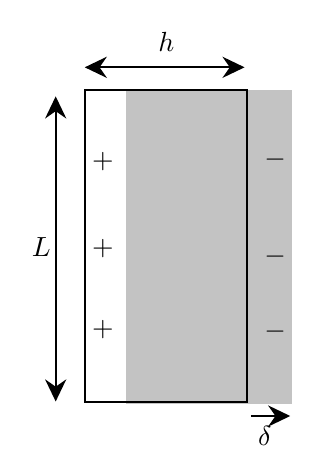
\begin{tikzpicture}[x=0.75pt,y=0.75pt,yscale=-1,xscale=1]
%uncomment if require: \path (0,300); %set diagram left start at 0, and has height of 300

%Shape: Rectangle [id:dp7217887277897033] 
\draw  [draw opacity=0][fill={rgb, 255:red, 155; green, 155; blue, 155 }  ,fill opacity=0.6 ] (199,96) -- (279,96) -- (279,247) -- (199,247) -- cycle ;
%Shape: Rectangle [id:dp49084866599960386] 
\draw   (179,96) -- (257,96) -- (257,246.4) -- (179,246.4) -- cycle ;
%Straight Lines [id:da592262187480596] 
\draw    (165,102) -- (165,243) ;
\draw [shift={(165,246)}, rotate = 270] [fill={rgb, 255:red, 0; green, 0; blue, 0 }  ][line width=0.08]  [draw opacity=0] (10.72,-5.15) -- (0,0) -- (10.72,5.15) -- (7.12,0) -- cycle    ;
\draw [shift={(165,99)}, rotate = 90] [fill={rgb, 255:red, 0; green, 0; blue, 0 }  ][line width=0.08]  [draw opacity=0] (10.72,-5.15) -- (0,0) -- (10.72,5.15) -- (7.12,0) -- cycle    ;
%Straight Lines [id:da1395939334945815] 
\draw    (182,85) -- (253,85) ;
\draw [shift={(256,85)}, rotate = 180] [fill={rgb, 255:red, 0; green, 0; blue, 0 }  ][line width=0.08]  [draw opacity=0] (10.72,-5.15) -- (0,0) -- (10.72,5.15) -- (7.12,0) -- cycle    ;
\draw [shift={(179,85)}, rotate = 0] [fill={rgb, 255:red, 0; green, 0; blue, 0 }  ][line width=0.08]  [draw opacity=0] (10.72,-5.15) -- (0,0) -- (10.72,5.15) -- (7.12,0) -- cycle    ;
%Straight Lines [id:da6778726697290913] 
\draw    (259,253) -- (275,253) ;
\draw [shift={(278,253)}, rotate = 180] [fill={rgb, 255:red, 0; green, 0; blue, 0 }  ][line width=0.08]  [draw opacity=0] (10.72,-5.15) -- (0,0) -- (10.72,5.15) -- (7.12,0) -- cycle    ;


% Text Node
\draw (181,124.4) node [anchor=north west][inner sep=0.75pt]    {$+$};
% Text Node
\draw (181,166.4) node [anchor=north west][inner sep=0.75pt]    {$+$};
% Text Node
\draw (181,205.4) node [anchor=north west][inner sep=0.75pt]    {$+$};
% Text Node
\draw (264,123.4) node [anchor=north west][inner sep=0.75pt]    {$-$};
% Text Node
\draw (264,170.4) node [anchor=north west][inner sep=0.75pt]    {$-$};
% Text Node
\draw (264,206.4) node [anchor=north west][inner sep=0.75pt]    {$-$};
% Text Node
\draw (261,256.4) node [anchor=north west][inner sep=0.75pt]    {$\delta $};
% Text Node
\draw (152,165.4) node [anchor=north west][inner sep=0.75pt]    {$L$};
% Text Node
\draw (213,66.4) node [anchor=north west][inner sep=0.75pt]    {$h$};


\end{tikzpicture}
\end{center}
Bằng cách đặt tấm vào một điện trường đều bên ngoài, tất cả các electron đều bị dịch đi một khoảng nhỏ $\delta$, sao cho $|\delta| \ll h$, và vuông góc với trục của phiến. Chúng ta giả sử rằng $n_i$ và $n_e$ là không đổi, điện trường ngoài không làm nhiễu loạn mạng tinh thể và hiệu ứng rìa có thể được bỏ qua.
\begin{enumerate}[1)]
   \item Tính điện trường gây ra bởi sự dịch chuyển của các electron.
    \item Tính năng lượng điện trường của hệ.
Bây giờ điện trường ngoài bị tắt đi, và “mạng electron” bắt đầu dao động quanh vị trí cân bằng của nó.
  \item Tìm chu kì dao động của hệ với giả sử rằng độ dịch là nhỏ $(\delta \ll h)$.
\end{enumerate}
  
\end{vd}
\begin{loigiai}
  \begin{enumerate}[1)]
    \item Ta giả sử rằng $\delta >0$, sự dịch chuyển của các eletron dẫn điện do tác động của điện trường ngoài sẽ gây ra phân bố mật độ điện tích trên phiến.
\begin{center}


\tikzset{every picture/.style={line width=0.75pt}} %set default line width to 0.75pt        

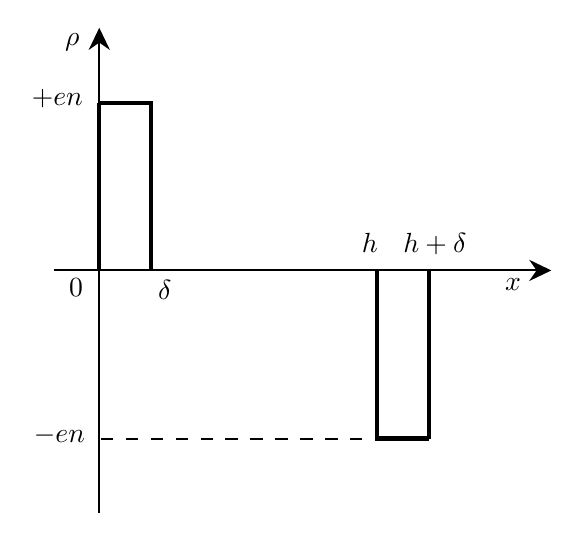
\begin{tikzpicture}[x=0.75pt,y=0.75pt,yscale=-1,xscale=1]
%uncomment if require: \path (0,300); %set diagram left start at 0, and has height of 300

%Straight Lines [id:da6451691314240162] 
\draw    (78,141) -- (314.8,141) ;
\draw [shift={(317.8,141)}, rotate = 180] [fill={rgb, 255:red, 0; green, 0; blue, 0 }  ][line width=0.08]  [draw opacity=0] (10.72,-5.15) -- (0,0) -- (10.72,5.15) -- (7.12,0) -- cycle    ;
%Straight Lines [id:da1410092498727764] 
\draw    (100,257.9) -- (100,27.1) ;
\draw [shift={(100,24.1)}, rotate = 450] [fill={rgb, 255:red, 0; green, 0; blue, 0 }  ][line width=0.08]  [draw opacity=0] (10.72,-5.15) -- (0,0) -- (10.72,5.15) -- (7.12,0) -- cycle    ;
%Straight Lines [id:da15557261132056954] 
\draw [line width=1.5]    (100,60.2) -- (100,141) ;
%Straight Lines [id:da9142755166526642] 
\draw [line width=1.5]    (124.8,60.2) -- (124.8,141) ;
%Straight Lines [id:da4536569984572141] 
\draw [line width=1.5]    (234,141.2) -- (234,222) ;
%Straight Lines [id:da69833388035731] 
\draw [line width=1.5]    (258.8,141.2) -- (258.8,222) ;
%Straight Lines [id:da14094267922415105] 
\draw [line width=1.5]    (100,60.2) -- (125.8,60.2) ;
%Straight Lines [id:da3546021934992991] 
\draw [line width=1.5]    (233,222) -- (258.8,222) ;
%Straight Lines [id:da5560792612540038] 
\draw  [dash pattern={on 4.5pt off 4.5pt}]  (100.8,222) -- (233,222) ;


% Text Node
\draw (66,52.4) node [anchor=north west][inner sep=0.75pt]    {$+en$};
% Text Node
\draw (67,214.4) node [anchor=north west][inner sep=0.75pt]    {$-en$};
% Text Node
\draw (82,25.4) node [anchor=north west][inner sep=0.75pt]    {$\rho $};
% Text Node
\draw (294,143.4) node [anchor=north west][inner sep=0.75pt]    {$x$};
% Text Node
\draw (225,121.4) node [anchor=north west][inner sep=0.75pt]    {$h$};
% Text Node
\draw (245,121.4) node [anchor=north west][inner sep=0.75pt]    {$h+\delta $};
% Text Node
\draw (126.8,144.4) node [anchor=north west][inner sep=0.75pt]    {$\delta $};
% Text Node
\draw (84,143.4) node [anchor=north west][inner sep=0.75pt]    {$0$};


\end{tikzpicture}
\end{center}
      \[\varrho (x) = \left\{ \begin{array}{cc}
      0, & x<0, \\
     +en, & 0<x<\delta,\\
              0, &  \delta<x<h, \\
     -en, &h<x< h+\delta, \\
     0, & x> h+\delta. \end{array}\right. \tag{1}\]

Điện trường gây ra bởi phân bố này có thể được tính bằng cách kết hợp phương trình $\nabla \cdot \ot{E} = \partial_x E_x = 4\pi k_{\mathrm{e}} \varrho$ và điều kiện biên $\ot{E}(-\infty) =0$:
      \[E_x(x) = 4\pi e n k_{\mathrm{e}} \left\{ \begin{array}{cc} 
                       0, & x<0, \\
                 x, & 0<x<\delta, \\
                 \delta , & \delta<x<h,\\
                   h+ \delta - x, & h<x<h+\delta , \\
              0, & x>h+\delta . 
            \end{array}\right. \tag{2} \]

  \begin{center}


\tikzset{every picture/.style={line width=0.75pt}} %set default line width to 0.75pt        

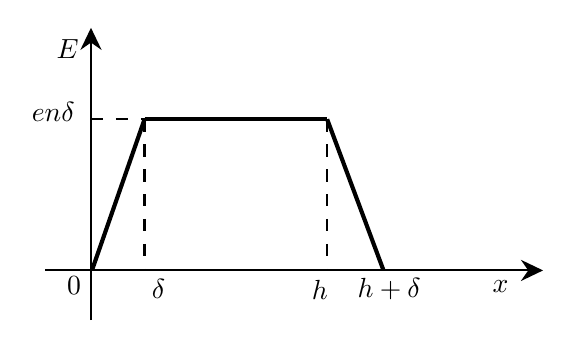
\begin{tikzpicture}[x=0.75pt,y=0.75pt,yscale=-1,xscale=1]
%uncomment if require: \path (0,300); %set diagram left start at 0, and has height of 300

%Straight Lines [id:da01641255710506151] 
\draw    (98,161) -- (334.8,161) ;
\draw [shift={(337.8,161)}, rotate = 180] [fill={rgb, 255:red, 0; green, 0; blue, 0 }  ][line width=0.08]  [draw opacity=0] (10.72,-5.15) -- (0,0) -- (10.72,5.15) -- (7.12,0) -- cycle    ;
%Straight Lines [id:da14878370163317478] 
\draw    (120,185) -- (120,47.1) ;
\draw [shift={(120,44.1)}, rotate = 450] [fill={rgb, 255:red, 0; green, 0; blue, 0 }  ][line width=0.08]  [draw opacity=0] (10.72,-5.15) -- (0,0) -- (10.72,5.15) -- (7.12,0) -- cycle    ;
%Straight Lines [id:da8675826770429016] 
\draw [line width=0.75]  [dash pattern={on 4.5pt off 4.5pt}]  (120,88.2) -- (145.8,88.2) ;
%Straight Lines [id:da9262762168352314] 
\draw [line width=0.75]  [dash pattern={on 4.5pt off 4.5pt}]  (145.8,88.2) -- (145.8,160.6) ;
%Straight Lines [id:da7374057248217938] 
\draw [line width=0.75]  [dash pattern={on 4.5pt off 4.5pt}]  (233.8,88.2) -- (233.8,160.6) ;
%Straight Lines [id:da034445088923599654] 
\draw [line width=1.5]    (145.8,88.2) -- (120.6,160.6) ;
%Straight Lines [id:da6877283104927654] 
\draw [line width=1.5]    (145.8,88.2) -- (233.8,88.2) ;
%Straight Lines [id:da6022831934893127] 
\draw [line width=1.5]    (233.8,88.2) -- (260.8,160.6) ;


% Text Node
\draw (102,48.4) node [anchor=north west][inner sep=0.75pt]    {$E$};
% Text Node
\draw (90,78.4) node [anchor=north west][inner sep=0.75pt]    {$en\delta $};
% Text Node
\draw (107,162.4) node [anchor=north west][inner sep=0.75pt]    {$0$};
% Text Node
\draw (147.8,164) node [anchor=north west][inner sep=0.75pt]    {$\delta $};
% Text Node
\draw (224.9,164.4) node [anchor=north west][inner sep=0.75pt]    {$h$};
% Text Node
\draw (247,163.4) node [anchor=north west][inner sep=0.75pt]    {$h+\delta $};
% Text Node
\draw (312,164.4) node [anchor=north west][inner sep=0.75pt]    {$x$};


\end{tikzpicture}
\end{center}
Nếu chúng ta giả sử độ dịch là âm $-\delta$ (với $\delta>0$) thì mật độ điện tích và điện trường là 

    \[\begin{aligned}
       \varrho(x) &= 
       \left\{\begin{array}{cc}
                                     0, & x<-\delta,  \\
                              -en, & -\delta <x<0,\\
                            0, &  0<x<h-\delta, \\
                          +en, &h-\delta<x< h, \\
                               0,      &x> h . 
                  \end{array}\right.\\
        E_x(x) &= 4\pi e n k_{\mathrm{e}}   
        \left\{\begin{array}{cc}
                                     0, & x<-\delta,  \\
                              -en, & -\delta <x<0,\\
                            0, &  0<x<h-\delta, \\
                          +en, &h-\delta<x< h, \\
                               0,      &x> h . 
                  \end{array}\right. 
    \end{aligned}\tag{3}\]

Đồ thị cho trường hợp này có thể thu được bằng cách đảo trục $x$ và chuyển $\delta$ sang phần âm của trục $x$.
\item Năng lượng tĩnh điện của hệ, trong trường hợp độ dịch là dương, có thể tính được bằng tích phân mật độ năng lượng $u={E_x}^2/(8\pi k_{\mathrm{e}})$ trên toàn bộ vùng không gian:
 \[\begin{aligned}
U_{\mathrm{es}} &=\int \frac{E_{x}^{2}}{8 \pi k_{\mathrm{e}}} \mathrm{d}^{3} r=\frac{L^{2}}{8 \pi k_{\mathrm{e}}} \int_{0}^{h+\delta} E_{x}^{2} \mathrm{~d} x \\
&=\frac{L^{2}}{8 \pi k_{\mathrm{e}}}(4 \pi e n k_{\mathrm{e}})^{2}\left[\int_{0}^{\delta} x^{2} \mathrm{~d} x+\int_{\delta}^{h} \delta^{2} \mathrm{~d} x+\int_{h}^{h+\delta}(h+\delta-x)^{2} \mathrm{~d} x\right] \\
&=2 \pi k_{\mathrm{e}}(e n L)^{2}\left[\frac{\delta^{3}}{3}+\delta^{2}(h-\delta)+\frac{\delta^{3}}{3}\right]=2 \pi k_{\mathrm{e}}(e n L)^{2}\left(h \delta^{2}-\frac{\delta^{3}}{3}\right),
\end{aligned} \tag{4} \]
ở đây, do tính đối xứng của hệ, chúng ta sử dụng $\dd^3 r = L^2 \dd x $. Kết quả tương tự cũng sẽ đạt được nếu chúng ta coi độ dịch là $-\delta$. Độ dịch $\delta$ xuất hiện ở cuối biểu thức $4)$ trên thực tế phải được viết là $|\delta|$.
\item Ở giới hạn $\delta \ll h$ chúng ta có thể bỏ qua số hạng bậc ba của $\delta$ ở phương trình $4)$, và xấp xỉ $U_{\mathrm{es}} \approx 2\pi k_{\mathrm{e}} (enL)^2 h \delta^2$, năng lượng này là thế năng của một dao động điều hòa. Lực tác dụng lên ``mạng electron'' là 
   \[F= - \frac{\partial U_{\mathrm{es}}}{\partial \delta} = - 4 \pi k_{\mathrm{e}} (enL)^2h\delta, \tag{5}\]
ở đây $\delta$ có thể là âm hoặc dương. Phương trình chuyển động của electron là 
   \[M\ddot{\delta} = F = -M\omega^2\delta, \tag{6}\]
ở đây $M= m_e nL^2h$ là tổng khối lượng electron dẫn của bản. Từ đây ta có
     \[\omega^2 = \frac{4\pi k_{\mathrm{e}} n e^2}{m_e} \equiv \omega_p^2, \tag{7}\]
trong đó $\omega_p$ được gọi là tần số plasma, là một tính chất nội tại của vật dẫn, chỉ phụ thuộc vào mật độ electron tự do.
\end{enumerate}
\end{loigiai}
\begin{vd}[Khung dây quay trong từ trường]
Một khung dây dẫn hình vuông cạnh $a$ có thể quay không ma sát quanh một trục quay cố định thẳng đứng, nằm trong mặt phẳng khung dây và đi qua tâm khung như hình vẽ. Trục quay cách điện với khung. Khung được đặt trong từ trường đều có $\ot{B}$ nằm ngang. Khi khung dây ở vị trí cân bằng, mặt phẳng của khung vuông góc với $\ot{B}$. Moment quán tính của khung đối với trục quay là $I$, độ tự cảm của khung là ${L}$, bỏ qua điện trở của khung. Tại thời điểm ${t}=0$, khi khung đang ở vị trí cân bằng người ta tác động để tức thời tạo ra cho khung tốc độ góc $\omega_{0}$.
\begin{center}
\tikzset{every picture/.style={line width=0.75pt}} %set default line width to 0.75pt        

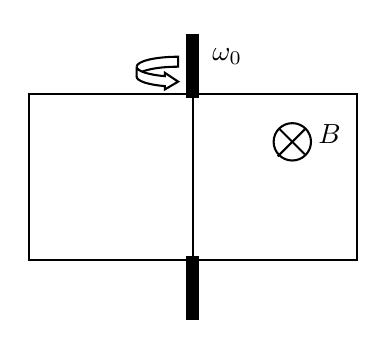
\begin{tikzpicture}[x=0.75pt,y=0.75pt,yscale=-1,xscale=1]
%uncomment if require: \path (0,300); %set diagram left start at 0, and has height of 300

%Shape: Rectangle [id:dp3627669737162238] 
\draw   (100,105) -- (258,105) -- (258,185) -- (100,185) -- cycle ;
%Straight Lines [id:da09761083232431433] 
\draw    (179,76) -- (179,214) ;
%Straight Lines [id:da3552654969304896] 
\draw [line width=4.5]    (179,76) -- (179,107) ;
%Straight Lines [id:da5995858710705217] 
\draw [line width=4.5]    (179,183) -- (179,214) ;
%Shape: Circle [id:dp16914754673779608] 
\draw   (218,128) .. controls (218,123.03) and (222.03,119) .. (227,119) .. controls (231.97,119) and (236,123.03) .. (236,128) .. controls (236,132.97) and (231.97,137) .. (227,137) .. controls (222.03,137) and (218,132.97) .. (218,128) -- cycle ;
%Straight Lines [id:da5982482411107883] 
\draw    (221,122) -- (233,134) ;
%Straight Lines [id:da8280335061260731] 
\draw    (233,122) -- (220,135) ;
%Curve Left Arrow [id:dp6091814054119917] 
\draw  [fill={rgb, 255:red, 255; green, 255; blue, 255 }  ,fill opacity=1 ] (152,91.8) .. controls (152,89.15) and (160.95,87) .. (172,87) -- (172,91.8) .. controls (160.95,91.8) and (152,93.95) .. (152,96.6) ;\draw  [fill={rgb, 255:red, 255; green, 255; blue, 255 }  ,fill opacity=1 ] (152,96.6) .. controls (152,98.71) and (157.69,100.51) .. (165.6,101.15) -- (165.6,102.75) -- (172,99) -- (165.6,94.75) -- (165.6,96.35) .. controls (157.69,95.71) and (152,93.91) .. (152,91.8)(152,96.6) -- (152,91.8) ;

% Text Node
\draw (238,118.4) node [anchor=north west][inner sep=0.75pt]    {$\ot B$};
% Text Node
\draw (187,81.4) node [anchor=north west][inner sep=0.75pt]    {$\omega _{0}$};


\end{tikzpicture}
\end{center}
\begin{enumerate}[1)]
\item Tính cường độ dòng điện cực đại qua khung.
\item Tìm điều kiện của tốc độ góc để khung quay không quá nửa vòng.
\end{enumerate}
\end{vd}

\begin{loigiai}\[\]
\begin{enumerate}[1)]
    \item 
Suất điện động xuất hiện trong khung:
\[
\begin{aligned}
e_{C} &= -\dfrac{\mathrm{d} \Phi}{\mathrm{d} t}=-\dfrac{\mathrm{d}\left(a^{2} B \cos \varphi\right)}{\mathrm{d} t} = a^{2} B \cdot \sin \varphi \cdot \dfrac{\mathrm{d} \varphi}{\mathrm{d} t}, \\
e_{C} &= a^{2} B \cdot \omega \sin \varphi.
\end{aligned}
\]
Suất điện động tự cảm trong khung:
\[
e_{tc}=-L \dfrac{\mathrm{d} i}{\mathrm{d} t}.
\]
Theo định luật Kirchhoff:
\[e_{C}+e_{t c}=iR=0.\] 
Do đó:
\[
L \dfrac{\mathrm{d} i}{\mathrm{d} t}=a^{2} B \cdot \omega \sin \varphi. \tag{1} \label{uu1}
\]
Phương trình chuyển động quay của khung:
\[
M = I \cdot \dfrac{\mathrm{d} \omega}{\mathrm{d} t} \Rightarrow -i B S \sin \varphi = I \cdot \dfrac{\mathrm{d} \omega}{\mathrm{d} t} \Rightarrow - i B a^{2} \sin \varphi = I \cdot \dfrac{\mathrm{d} \omega}{\mathrm{d} t}. \tag{2} \label{uu2}
\]
Từ (\ref{uu1}) và (\ref{uu2}) suy ra:
\[i \mathrm{d}i=-\dfrac{I}{L} \cdot \omega \mathrm{d} \omega.\]
Lấy tích phân hai vế:
\begin{align*}
\int_{0}^{i} i \cdot \mathrm{d} i=-\dfrac{I}{L} \cdot \int_{\omega_{0}}^{\omega} \omega \mathrm{d} \omega,\\
\Rightarrow i^{2}=\dfrac{I}{L}\left(\omega_{0}^{2}-\omega^{2}\right).  
\end{align*}
\[\Rightarrow i_{\max }=\omega_{0} \sqrt{\dfrac{I}{L}}\text{(ứng với $\omega=0$).}\]
\item Từ (\ref{uu1}):
\[\dfrac{L}{a^{2} B} \mathrm{d} i=(\omega \sin \varphi) \cdot \mathrm{d} t=\sin \varphi \cdot \mathrm{d} \varphi.\]
Tích phân hai vế:
\[\Rightarrow 1-\cos \varphi_{\max }=\dfrac{L}{a^{2} B} i_{\max }=\dfrac{\sqrt{L I}}{a^{2} B} \omega_{0} \Rightarrow \cos \varphi_{\max }=1-\dfrac{\sqrt{L I}}{a^{2} B} \omega_{0}\]
Để khung quay không quá nửa vòng thì:
\[\varphi_{\max } \leq \pi \Rightarrow \cos \varphi_{\max } \geq-1 \Rightarrow \omega_{0} \leq 2\dfrac{a^{2} B}{\sqrt{L I}}.\]
\end{enumerate}
\end{loigiai}
\begin{vd}[*]\textbf{Cặp electrons và điện trường}\\
Ở đây chúng ta nghiên cứu chuyển động của hai electron trong mặt phẳng vuông góc với các đường sức của một từ trường đều. Hai electron được coi gần đúng như các chất điểm cổ điển và chỉ chịu tác dụng của lực điện và lực từ.
\begin{enumerate}[1)]
    \item Ban đầu hai electron đứng yên và cách nhau một khoảng là $d$. Chúng được truyền các vận tốc đầu cùng độ lớn $v$ nhưng ngược chiều nhau. Tìm điều kiện của $d$ để sau khi bắt đầu chuyển động, khoảng cách giữa chúng luôn là hằng số. Tìm biểu thức của $d$ lúc này.
    \item Chứng tỏ rằng có thể duy trì khoảng cách không đổi $d$ chỉ bằng cách truyền vận tốc cho một electron.Tìm quỹ đạo của khối tâm hệ trong trường hợp này. Vẽ phác họa quỹ đạo chuyển động của các electron. Khi nào thì electron ban đầu chuyển động sẽ dừng.
\end{enumerate}
\end{vd}
\begin{loigiai}
    \begin{enumerate}[1)]
        \item Để khoảng cách là không đổi, hai electron phải chuyển động cùng quỹ đạo trên cùng một đường tròn với bán kính $d/2$; chúng phải nằm đối xứng nhau qua tâm hình tròn và chuyển động với cùng vận tốc $v$ (như hình vẽ). Cả hai electron chuyển động trong từ trường đều chịu tác dụng của lực Lorentz và lực đẩy tĩnh điện giữa chúng tổng hợp lại thành một lực hướng tâm giữ cho chúng chuyển động thẳng đều.
        \begin{center}
            \tikzset{every picture/.style={line width=0.75pt}} %set default line width to 0.75pt        
            \begin{tikzpicture}[x=0.75pt,y=0.75pt,yscale=-1,xscale=1]
            %uncomment if require: \path (0,521); %set diagram left start at 0, and has height of 521
            
            %Shape: Ellipse [id:dp37933654197498545] 
            \draw   (166.08,212.4) .. controls (166.08,156.95) and (211.03,112) .. (266.48,112) .. controls (321.93,112) and (366.88,156.95) .. (366.88,212.4) .. controls (366.88,267.85) and (321.93,312.8) .. (266.48,312.8) .. controls (211.03,312.8) and (166.08,267.85) .. (166.08,212.4) -- cycle ;
            %Shape: Ellipse [id:dp020176206185545054] 
            \draw  [fill={rgb, 255:red, 0; green, 0; blue, 0 }  ,fill opacity=1 ] (161.72,212.4) .. controls (161.72,209.99) and (163.67,208.03) .. (166.08,208.03) .. controls (168.49,208.03) and (170.45,209.99) .. (170.45,212.4) .. controls (170.45,214.81) and (168.49,216.77) .. (166.08,216.77) .. controls (163.67,216.77) and (161.72,214.81) .. (161.72,212.4) -- cycle ;
            %Shape: Ellipse [id:dp7333140222111905] 
            \draw  [fill={rgb, 255:red, 0; green, 0; blue, 0 }  ,fill opacity=1 ] (362.52,212.4) .. controls (362.52,209.99) and (364.47,208.03) .. (366.88,208.03) .. controls (369.29,208.03) and (371.25,209.99) .. (371.25,212.4) .. controls (371.25,214.81) and (369.29,216.77) .. (366.88,216.77) .. controls (364.47,216.77) and (362.52,214.81) .. (362.52,212.4) -- cycle ;
            %Straight Lines [id:da5858758890164644] 
            \draw    (166.08,208.03) -- (166.08,165.68) ;
            \draw [shift={(166.08,163.68)}, rotate = 450] [color={rgb, 255:red, 0; green, 0; blue, 0 }  ][line width=0.75]    (10.93,-3.29) .. controls (6.95,-1.4) and (3.31,-0.3) .. (0,0) .. controls (3.31,0.3) and (6.95,1.4) .. (10.93,3.29)   ;
            %Straight Lines [id:da6699826148149972] 
            \draw    (166.08,212.4) -- (226.94,212.4) ;
            \draw [shift={(228.94,212.4)}, rotate = 180] [color={rgb, 255:red, 0; green, 0; blue, 0 }  ][line width=0.75]    (10.93,-3.29) .. controls (6.95,-1.4) and (3.31,-0.3) .. (0,0) .. controls (3.31,0.3) and (6.95,1.4) .. (10.93,3.29)   ;
            %Straight Lines [id:da12871600619765244] 
            \draw    (367.75,212.4) -- (399.8,212.4) ;
            \draw [shift={(401.8,212.4)}, rotate = 180] [color={rgb, 255:red, 0; green, 0; blue, 0 }  ][line width=0.75]    (10.93,-3.29) .. controls (6.95,-1.4) and (3.31,-0.3) .. (0,0) .. controls (3.31,0.3) and (6.95,1.4) .. (10.93,3.29)   ;
            %Straight Lines [id:da33537398216713554] 
            \draw    (366.88,212.4) -- (308.64,212.4) ;
            \draw [shift={(306.64,212.4)}, rotate = 360] [color={rgb, 255:red, 0; green, 0; blue, 0 }  ][line width=0.75]    (10.93,-3.29) .. controls (6.95,-1.4) and (3.31,-0.3) .. (0,0) .. controls (3.31,0.3) and (6.95,1.4) .. (10.93,3.29)   ;
            %Straight Lines [id:da39133811789746975] 
            \draw    (166.08,212.4) -- (133.16,212.4) ;
            \draw [shift={(131.16,212.4)}, rotate = 360] [color={rgb, 255:red, 0; green, 0; blue, 0 }  ][line width=0.75]    (10.93,-3.29) .. controls (6.95,-1.4) and (3.31,-0.3) .. (0,0) .. controls (3.31,0.3) and (6.95,1.4) .. (10.93,3.29)   ;
            %Straight Lines [id:da8153194046125287] 
            \draw    (366.88,212.4) -- (366.88,265.58) ;
            \draw [shift={(366.88,267.58)}, rotate = 270] [color={rgb, 255:red, 0; green, 0; blue, 0 }  ][line width=0.75]    (10.93,-3.29) .. controls (6.95,-1.4) and (3.31,-0.3) .. (0,0) .. controls (3.31,0.3) and (6.95,1.4) .. (10.93,3.29)   ;
            %Straight Lines [id:da11308212969163933] 
            \draw    (266.48,212.4) -- (305.31,299.8) ;
            \draw [shift={(306.12,301.63)}, rotate = 246.05] [color={rgb, 255:red, 0; green, 0; blue, 0 }  ][line width=0.75]    (10.93,-3.29) .. controls (6.95,-1.4) and (3.31,-0.3) .. (0,0) .. controls (3.31,0.3) and (6.95,1.4) .. (10.93,3.29)   ;
            %Shape: Circle [id:dp5670320230480146] 
            \draw   (224.58,170.06) .. controls (224.58,165.38) and (228.37,161.59) .. (233.04,161.59) .. controls (237.72,161.59) and (241.51,165.38) .. (241.51,170.06) .. controls (241.51,174.73) and (237.72,178.53) .. (233.04,178.53) .. controls (228.37,178.53) and (224.58,174.73) .. (224.58,170.06) -- cycle ;
            %Straight Lines [id:da8344401093990392] 
            \draw [line width=1.5]    (228.69,166.45) -- (237.02,174.78) ;
            %Straight Lines [id:da8741424678522312] 
            \draw [line width=1.5]    (237.02,166.45) -- (228.61,174.86) ;
            
            
            
            % Text Node
            \draw (242.96,146.8) node [anchor=north west][inner sep=0.75pt]    {$\ot{B}$};
            % Text Node
            \draw (152.16,169.01) node [anchor=north west][inner sep=0.75pt]    {$v$};
            % Text Node
            \draw (367.8,241.99) node [anchor=north west][inner sep=0.75pt]    {$v$};
            % Text Node
            \draw (186.64,192.45) node [anchor=north west][inner sep=0.75pt]    {$F_{L}$};
            % Text Node
            \draw (328.94,192.45) node [anchor=north west][inner sep=0.75pt]    {$F_{L}$};
            % Text Node
            \draw (136.37,191.58) node [anchor=north west][inner sep=0.75pt]    {$F_{C}{}_{b}$};
            % Text Node
            \draw (370.34,190.7) node [anchor=north west][inner sep=0.75pt]    {$F_{C}{}_{b}$};
            % Text Node
            \draw (290.04,227.85) node [anchor=north west][inner sep=0.75pt]    {$\dfrac{d}{2}$};
            \end{tikzpicture}
        \end{center}
    Chúng ta viết phương trình chuyển động cho một electron. Lực lorentz tác dụng lên một hạt với điện tích $-e$, khối lượng $m$ và vận tốc $v$ là 
    \[F_L=evB,\]
    và lực đẩy Coulomb giữa hai electron \[F_{Cb}=k_{\mathrm{e}}\dfrac{e^2}{d^2}.\]
    Lực Coulomb luôn là lực đẩy và vì lực Lorentz luôn vuông góc với vận tốc nên cả hai lực này đều theo phương xuyên tâm so với quỹ đạo của hạt. 
    \\ \textbf{Chú ý:} Trên lí thuyết chúng ta phải tính thêm cả lực từ do từ trường của electron chuyển động gây ra (và có thể tính được thông qua định lí Biot-Savart):
         \[F_{\mathrm{magn}}=e v \frac{\mu_{0}}{4 \pi} \frac{e v}{d^{2}}=\frac{v^{2}}{c^{2}} F_{\mathrm{Cb}},\]
    trong đó $c$ là vận tốc ánh sáng trong chân không. Tuy nhiên trong giới hạn của cơ học cổ điển phi tương đối tính, $v\ll c$, lực này là không đáng kể so với lực Coulomb. Do đó chúng ta bỏ qua lực này.
    Phương trình chuyển động của electron do đó là
        \[evB-k_{\mathrm{e}}\dfrac{e^2}{d^2}=m\dfrac{v^2}{d/2}.\]
    Đây là một phương trình bậc hai của $v$, và các nghiệm của nó là
        \[v=\dfrac{edB}{4m} \pm \sqrt{\left(\dfrac{edB}{4m}\right)^2-\dfrac{k_{\mathrm{e}}e^2}{2md}}.\]
    Điều kiện để bài có thể thỏa mãn nếu như vận tốc thu được là số thực và dương, do đó biểu thức trong căn phải là dương. Do đó ta thu được điều kiện của $d$ là 
        \[d \geqslant 2\sqrt[3]{{\frac{{{k_{\mathrm{e}}}m}}{{{B^2}}}}} = {d_{\mathrm{crit}}}.\]
    Nếu các electron gần nhau hơn khoảng cách giới hạn, chúng ta sẽ không tìm được nghiệm. Nếu khoảng cách đúng bằng khoảng cách giới hạn, ta thu được nghiệm duy nhất. Còn nếu khoảng cách lớn hơn $d_{crit}$, chúng ta luôn thu được hai nghiệm vận tốc thỏa mãn. 
    
      \item Nếu chỉ một electron được cung cấp vận tốc đầu, chuyển động sẽ trở nên phức tạp hơn, kể cả đối với trường hợp đặc biệt của đề bài, đó là khoảng cách của 2 electron là không đổi. \\
   Chúng ta có thể tiếp cận gần hơn với lời giải khi xử lí được câu hỏi phụ trợ ``quỹ đạo của khối tâm hệ lúc này như nào?'' \\
   Dùng các phương trình vector cơ bản của chuyển động ta có:
   \[m \ot{a_1} = k_{\mathrm{e}} \dfrac{e^{2}}{\left|\ot{r_1}- \ot{r_2}\right|^{3}}\left(\ot{r_1}-\ot{r_2}\right)-e \ot{v_1} \times \ot{B}, \tag{1}\label{N.5.1}\]
    \[m \ot{a_2} = k_{\mathrm{e}} \dfrac{e^{2}}{\left|\ot{r_1}-\ot{r_2}\right|^{3}}\left(\ot{r_2}-\ot{r_1}\right)-e \ot{v_2} \times \ot{B}. \tag{2}\label{N.5.2} \]
    Với hai hạt có cùng khối lượng, chúng ta có thể công nhận
    \[\ot{r_{\mathrm{CM}}}=\frac{\ot{r_1}+\ot{r_2}}{2}, \quad \ot{v_{\mathrm{CM}}}=\dfrac{\ot{v_1}+\ot{v_2}}{2}, \quad \ot{a_{\mathrm{CM}}}=\dfrac{\ot{a_1}+\ot{a_2}}{2}.\]
     Và phương trình chuyển động tổng quát của cả hai hạt
     \[m\left(\ot{a_1}+\ot{a_2}\right) = 0-e\left(\ot{v_1}+\ot{v_2}\right) \times \ot{B},\]
     Từ đó, ta dẫn ra 
     \[m \ot{a_\mathrm{CM}}=-e \ot{v_\mathrm{CM}} \times \ot{B}.\]
      Đối với hệ khối tâm, tương tác Coulomb nội tại đã được triệt tiêu.\\
    Phương trình cuối cùng là tiền đề để ta kết luận rằng khối tâm của hệ hai electron chuyển động trong từ trường tương tự như một electron duy nhất. Nếu từ trường là đều và chuyển động vuông góc với các đường sức từ, thì khối tâm của hệ chuyển động với quỹ đạo tròn đều!\\
    Chúng ta kết luận rằng khối tâm chuyển động tròn đều, còn hai electron ``dao động'' quanh quỹ đạo đó. Vận tốc góc của khối tâm là:
    \[\omega_{\mathrm{CM}}=\dfrac{a_{\mathrm{CM}}}{v_{\mathrm{CM}}}=\dfrac{e}{m} B=\omega_{\mathrm{c}}.\]
    Kết quả này cũng giống tần số cyclotron của electron $-$ vận tốc góc của các electron trong các máy gia tốc hạt. Bán kính của quỹ đạo khối tâm là
    \[R_{\mathrm{CM}}=\dfrac{v_{\mathrm{CM}}}{\omega_{\mathrm{CM}}}=\dfrac{v_{\mathrm{CM}}}{\omega_{\mathrm{c}}}.\]
    Thế các electron chuyển động xung quanh khối tâm như nào? Lời giải cho câu hỏi này cũng chính là đáp số cuối cùng của bài toán. Chúng ta viết vector độ dời của electron $1$ là $\ot{r_1} =\ot{r_\mathrm{CM}}+\ot{R}$. Do đó vector độ dời của electron 2 là $\ot{r_2} = \ot{r_\mathrm{CM}} - \ot{R}$. Dùng định nghĩa khối tâm ta có
    \[\ot{R}=\ot{r_1}-\ot{r_\mathrm{CM}}=\ot{r_1}-\dfrac{\ot{r_1}+\ot{r_2}}{2}=\dfrac{\ot{r_1}-\ot{r_2}}{2}.\]
     Một phương trình về sự thay đổi của vector này theo thời gian có thể được dẫn ra từ sự khác biệt giữa phương trình (\ref{N.5.1}) và (\ref{N.5.2})
     \[m\left(\ot{a_1}-\ot{a_2}\right)=2 k_{\mathrm{e}} \dfrac{e^{2}}{\left|\ot{r_1}-\ot{r_2}\right|^{3}}\left(\ot{r_1}-\ot{r_2}\right)-e\left[\left(\ot{v_1}-\ot{v_2}\right) \times \ot{B}\right].\tag{3}\label{N.5.3}\]
     Sự khác biệt của hai vector độ dời chính là $2$ lần vector $\ot R$ ở trên; do đó sự khác biệt về vận tốc chính là $2$ lần vector $\ot V$ (độ thay đổi của vector $\ot R$ theo thời gian). Và suy luận tương tự cũng được áp dụng với gia tốc.
     \[\ot{r_1} - \ot{r_2} =2 \ot{R}, \quad \ot{v_1}-\ot{v_2}=2 \ot{V}, \quad \ot{a_1}-\ot{a_2}=2 \ot{A}.\]
    Dùng bổ chính này, phương trình (\ref{N.5.3}) có thể được viết lại thành:
    \[m \ot{A}=k_{\mathrm{e}} \dfrac{e^{2}}{\left|2 \ot{R}\right|^{3}} 2 \ot{R} - e \tron{\ot{V} \times \ot{B}}. \tag{4}\label{N.5.4}\]
     Phương trình chuyển động này nội tại tương tự với phương trình ở câu $1)$, khi mà khối tâm của hệ đứng yên, do đó phương trình này cũng có nghiệm là chuyển động tròn đều.\\
   Công nhận dạng nghiệm của phương trình, nếu độ lớn của vector $\ot{R}(t)$ không thay đổi theo thời gian với giá trị $R$, và hướng của nó quay với vận tốc góc $\omega$, áp dụng phương trình của chuyển động tròn đều, ta có
    \[A=-\omega^{2} R \ {\text { và }} \  \ot{V} \times \ot{B}=R \omega B.\]
    Và từ phương trình (\ref{N.5.4}), chúng ta thu được phương trình bậc hai cho vận tốc góc $\omega$ của cặp electron, khi chúng quay quanh khối tâm:
    \[\omega^{2}-\dfrac{e}{m} B \omega + \dfrac{k_{\mathrm{e}}}{m} \dfrac{e^{2}}{4 R^{3}}=0. \tag{5}\label{N.5.5}\]
    Nghiệm thực của phương trình xuất hiện khi biểu thức $\Delta$ không âm, tức là
    \[R \geq \sqrt[3]{\dfrac{k_{\mathrm{e}} m}{B^{2}}}.\] 
      Lúc này khoảng cách tối thiểu giữa hai electron là 
      \[d_{\min }=2 R_{\min }=2 \sqrt[3]{\dfrac{k_{\mathrm{e}} m}{B^{2}}}=d_{\text{crit}}.\]
    Tất cả các lập luận của chúng ta đều thỏa mãn kể cả khi khối tâm của hệ không chuyển động, do đó không có gì bất ngờ khi giá trị của $d_{\mathrm{crit}}$ là giống hệt trong phần $1)$.\\
     Chúng ta sẽ phác họa quỹ đạo của hai electron trong trường hợp $d = d_{\min}$, khi đó
     \[R=R_{\min}=\sqrt[3]{\dfrac{k_{\mathrm{e} } m}{B^{2}}}.\]
     
     Thay giá trị này vào phương trình (\ref{N.5.5}), ta thu được vận tốc góc của hai electron chuyển động quanh khối tâm
    \[\omega = \dfrac{1}{2} \dfrac{e}{m} B=\dfrac{1}{2} \omega_{\mathrm{c}}.\]
    Giá trị của vận tốc góc này đúng bằng một nửa giá trị vận tốc góc của khối tâm.\\
   Kích thích hệ, như mô tả của ý $2)$, một electron được cấp vận tốc ban đầu $v_0$. Vận tốc này phải vuông góc với đường nối tâm của hai electron, nếu không khoảng cách giữa chúng sẽ thay đổi ngay tức thì sau đó.\\
   Ban đầu electron thứ $2$ sẽ ở trạng thái đứng yên và khối tâm chuyển động với vận tốc $v_0/2$, do đó vận tốc của mỗi electron đối với khối tâm có độ lớn bằng nhau nhưng ngược hướng.\\
   Với chuyển động tròn quanh khối tâm, ta có 
    \[\dfrac{v_0}{2} = R\omega = R \dfrac{\omega_{\mathrm{c}}}{2}.\]
    Đồng thời, với chuyển động tròn của khối tâm, ta có
    \[\dfrac{v_{0}}{2} = R_{\mathrm{CM}} \omega_{\mathrm{c}}, \ \text{ nên }  \ R_{\mathrm{CM}}=\dfrac{R}{2}.\]
     Do đó, electron chuyển động tròn quanh khối tâm với một quỹ đạo có bán kính gấp đôi bán kính chuyển động tròn của khối tâm. Hơn nữa chu kì quay của khối tâm bằng một nửa chu kì của electron quay quanh nó.\\
     Hình vẽ phác họa của quỹ đạo electron như trên hình $2$. Để dễ hình dung hơn, chúng ta thêm vào cả quỹ đạo của khối tâm electron (được vẽ bằng các nét đứt). Khi đường nối electron quay được một góc $\theta$ quanh khối tâm thì khối tâm đã quay được một góc $2 \theta$ trên quỹ đạo riêng của nó, với bán kính quỹ đạo bằng một nửa.

    \begin{center}
        \includegraphics[scale=0.75]{Anh/Nam4.pdf}\\
        Hình $2$.
    \end{center}
     Sau một chu kì $T = \dfrac{2\pi}{\omega_{\mathrm{c}}}$, khối tâm hoàn thành một vòng quay của nó, nhưng mỗi electron chỉ đi được nửa vòng; và do đó chúng đổi vị trí cho nhau. Tại thời điểm đó, vị trí và vận tốc của khối tâm giống hệt như lúc bắt đầu chuyển động $(v_0/2)$, electron ban đầu đứng yên có vận tốc $v_0$ và electron được kích thích bây giờ đứng yên. Nó dừng lại lần đầu tiên sau 
     \[T = 2\pi \dfrac{m}{eB}.\]
    \textbf{Mở rộng:}
    \begin{enumerate}[1)]
        \item Quỹ đạo chuyển động của hai eletron (được gọi là đường cardioid hay đường “trái tim”, do hình dạng đặc biệt của nó) chỉ đơn giản và đơn điệu chỉ khi khoảng cách ban đầu giữa các $e$ bằng khoảng cách giới hạn với từ trường cho trước. Nếu khoảng cách giữa chúng lớn hơn khoảng cách giới hạn, lúc đó quỹ đạo và chuyển động của các electron không đơn giản nữa, và nhìn chung quỹ đạo lúc này sẽ là quỹ đạo mở (điểm bắt đầu và kết thúc chu kì không trùng nhau).
        \item Bài toán sẽ càng phức tạp nếu vận tốc ban đầu không thỏa mãn điều kiện khoảng cách không đổi. Nhưng kể cả khi đó ta có thể chứng minh rằng hai electron không thể tiến tới quá gần nhau cũng như rời quá xa nhau, do đó khoảng cách giữa chúng sẽ dao động giữa hai giá trị giới hạn.
    \end{enumerate}
        
    \end{enumerate}
\end{loigiai}
\begin{vd}\textbf{VPhO 2018}\\
Một linh kiện điện tử có cấu tạo gồm một cathode $K$ dạng sợi dây dẫn mảnh, thẳng, dài và một anôt $A$ dạng trụ rỗng, có bán kính ${R}$, bao quanh cathode và có trục trùng với cathode. Linh kiện đặt trong không gian có từ trường đều $\ot{B}$ hướng dọc theo cathode. Bằng một cách nào đó, người ta tạo một điện trường $\ot{E}$ hướng trục từ ${A}$ đến ${K}$ có độ lớn không đổi.\\
Do tính đối xứng trục của bài toán, ta xét một hệ tọa độ trụ như hình. Hệ tọa độ được chọn sao cho gốc ${O}$ nằm trên ${K}$, trục ${Oz}$ theo chiều $\ot{B}$, từ trường $\ot{B}=\left(B_{\rho}, B_{\theta}, B_{z}\right)=(0,0, B)$
và điện trường
$$\ot{E}=\left(E_{\rho}, E_{\theta}, E_{z}\right)=(E, 0,0).$$ 
Khi cathode ${K}$ được đốt nóng sẽ bức xạ electron. Coi vận tốc của các electron phát ra từ cathode ${K}$ là rất nhỏ và bỏ qua tác dụng của trọng lực lên các electron này. Khi xem xét chuyển động của electron, không gian trong linh kiện có thể coi là chân không.
\begin{center}
{
\tikzset{every picture/.style={line width=0.75pt}} %set default line width to 0.75pt        

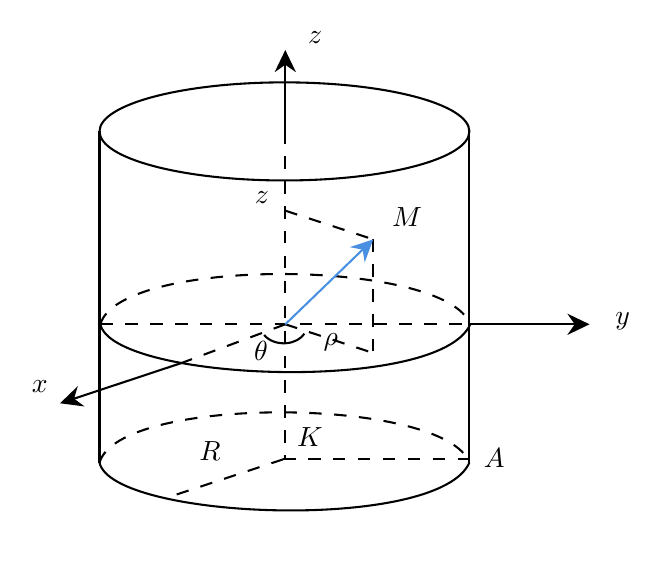
\begin{tikzpicture}[x=0.75pt,y=0.75pt,yscale=-1,xscale=1]
%uncomment if require: \path (0,474); %set diagram left start at 0, and has height of 474

%Shape: Ellipse [id:dp991714530186085] 
\draw   (223.14,115.72) .. controls (223.14,102.67) and (263.03,92.09) .. (312.24,92.09) .. controls (361.45,92.09) and (401.34,102.67) .. (401.34,115.72) .. controls (401.34,128.77) and (361.45,139.35) .. (312.24,139.35) .. controls (263.03,139.35) and (223.14,128.77) .. (223.14,115.72) -- cycle ;
%Straight Lines [id:da5090442830728876] 
\draw    (223.14,115.72) -- (223.14,275.3) ;
%Curve Lines [id:da8521350306505784] 
\draw  [dash pattern={on 4.5pt off 4.5pt}]  (223.55,208.65) .. controls (232.86,175.87) and (389.76,176.83) .. (401.75,208.65) ;
%Curve Lines [id:da6280284607936966] 
\draw    (223.55,208.65) .. controls (229.55,236.18) and (387.07,242.39) .. (401.75,208.65) ;
%Curve Lines [id:da06707199242837247] 
\draw  [dash pattern={on 4.5pt off 4.5pt}]  (223.14,275.3) .. controls (232.44,242.52) and (389.35,243.47) .. (401.34,275.3) ;
%Curve Lines [id:da3349004032829275] 
\draw    (223.14,275.3) .. controls (229.14,302.83) and (386.66,309.04) .. (401.34,275.3) ;
%Straight Lines [id:da40853559092842495] 
\draw    (401.34,115.72) -- (401.34,275.3) ;
%Straight Lines [id:da6012789690231846] 
\draw  [dash pattern={on 4.5pt off 4.5pt}]  (223.55,208.65) -- (401.75,208.65) ;
%Straight Lines [id:da565528652758621] 
\draw    (401.75,208.65) -- (456.22,208.65) ;
\draw [shift={(459.22,208.65)}, rotate = 180] [fill={rgb, 255:red, 0; green, 0; blue, 0 }  ][line width=0.08]  [draw opacity=0] (10.72,-5.15) -- (0,0) -- (10.72,5.15) -- (7.12,0) -- cycle    ;
%Straight Lines [id:da9860459074898706] 
\draw  [dash pattern={on 4.5pt off 4.5pt}]  (312.65,115.72) -- (312.65,273.71) ;
%Straight Lines [id:da37175075777238975] 
\draw    (312.65,79.49) -- (312.65,115.72) ;
\draw [shift={(312.65,76.49)}, rotate = 90] [fill={rgb, 255:red, 0; green, 0; blue, 0 }  ][line width=0.08]  [draw opacity=0] (10.72,-5.15) -- (0,0) -- (10.72,5.15) -- (7.12,0) -- cycle    ;
%Straight Lines [id:da6837228115665901] 
\draw  [dash pattern={on 4.5pt off 4.5pt}]  (312.65,208.65) -- (262.68,227.29) ;
%Straight Lines [id:da5422064545392717] 
\draw    (262.68,227.29) -- (206.97,245.77) ;
\draw [shift={(204.12,246.71)}, rotate = 341.65] [fill={rgb, 255:red, 0; green, 0; blue, 0 }  ][line width=0.08]  [draw opacity=0] (10.72,-5.15) -- (0,0) -- (10.72,5.15) -- (7.12,0) -- cycle    ;
%Straight Lines [id:da17772674300232527] 
\draw  [dash pattern={on 4.5pt off 4.5pt}]  (311.62,273.71) -- (401.34,273.71) ;
%Straight Lines [id:da7646362348207041] 
\draw  [dash pattern={on 4.5pt off 4.5pt}]  (311.62,273.71) -- (254.7,292.49) ;
%Straight Lines [id:da9590432766813448] 
\draw  [dash pattern={on 4.5pt off 4.5pt}]  (312.65,208.65) -- (355.03,222.47) ;
%Straight Lines [id:da5777038896986804] 
\draw  [dash pattern={on 4.5pt off 4.5pt}]  (312.65,153.91) -- (355.03,167.73) ;
%Straight Lines [id:da5586061217127374] 
\draw  [dash pattern={on 4.5pt off 4.5pt}]  (355.03,167.73) -- (355.03,222.47) ;
%Straight Lines [id:da9883977422064121] 
\draw [color={rgb, 255:red, 74; green, 144; blue, 226 }  ,draw opacity=1 ]   (312.65,208.65) -- (352.87,169.81) ;
\draw [shift={(355.03,167.73)}, rotate = 496] [fill={rgb, 255:red, 74; green, 144; blue, 226 }  ,fill opacity=1 ][line width=0.08]  [draw opacity=0] (10.72,-5.15) -- (0,0) -- (10.72,5.15) -- (7.12,0) -- cycle    ;
%Shape: Arc [id:dp20863658466452928] 
\draw  [draw opacity=0] (321.86,213.17) .. controls (320.24,215.56) and (317.19,217.33) .. (313.45,217.73) .. controls (308.96,218.21) and (304.72,216.57) .. (302.44,213.81) -- (311.91,209.17) -- cycle ; \draw   (321.86,213.17) .. controls (320.24,215.56) and (317.19,217.33) .. (313.45,217.73) .. controls (308.96,218.21) and (304.72,216.57) .. (302.44,213.81) ;

% Text Node
\draw (470.17,201.29) node [anchor=north west][inner sep=0.75pt]    {$y$};
% Text Node
\draw (322.16,66.24) node [anchor=north west][inner sep=0.75pt]    {$z$};
% Text Node
\draw (296.52,143.26) node [anchor=north west][inner sep=0.75pt]    {$z$};
% Text Node
\draw (189.03,234.18) node [anchor=north west][inner sep=0.75pt]    {$x$};
% Text Node
\draw (269.77,263.67) node [anchor=north west][inner sep=0.75pt]    {$R$};
% Text Node
\draw (316.9,256.99) node [anchor=north west][inner sep=0.75pt]    {$K$};
% Text Node
\draw (362.57,150.9) node [anchor=north west][inner sep=0.75pt]    {$M$};
% Text Node
\draw (406.86,267.17) node [anchor=north west][inner sep=0.75pt]    {$A$};
% Text Node
\draw (296.15,215.37) node [anchor=north west][inner sep=0.75pt]    {$\theta $};
% Text Node
\draw (329.6,211.82) node [anchor=north west][inner sep=0.75pt]    {$\rho $};
\end{tikzpicture}
}\end{center}
Kí hiệu điện tích nguyên tố là $e$ và khối lượng electron là $m_{e}$. Giả sử ở thời điểm $t=0$ electron có tọa độ $\left(0,0, z_{0}\right)$, ở thời điểm $t>0$ electron ở tọa độ $(\rho, \theta, z)$, hãy:
\begin{enumerate}[1)]
    \item Viết các phương trình vi phân mô tả chuyển động của electron.
    \item Tìm phương trình quỹ đạo của electron.
    \item Tìm vận tốc dài của electron tại thời điểm $t$ bất kì.
\end{enumerate}
Cho biết trong hệ tọa độ trụ:
\begin{itemize}
    \item Chất điểm $M$ xác định bởi vector tọa độ $\overrightarrow{OM} = (\rho, \theta, z)$ có vận tốc và gia tốc tương ứng là $\ot{v}=(\dot{\rho}, \rho \dot{\theta}, \dot{z})$ và $\ot{a}=\left(\ddot{\rho}-\rho \dot{\theta}^{2}, \dfrac{1}{\rho} \dfrac{\dd}{\dd t}\left(\rho^{2} \dot{\theta}\right), \ddot{z}\right)$.
    \item Nếu $\ot{a}=\left(a_{\rho}, a_{\theta}, a_{z}\right), \ot{b}=\left(b_{\rho}, b_{\theta}, b_{z}\right)$ thì $$\ot{a}\times\ot{b}=\left(a_{\theta} b_{z}-a_{z} b_{\theta}, a_{z} b_{\rho}-a_{\rho} b_{z}, a_{\rho} b_{\theta}-a_{\theta} b_{\rho}\right)$$
\end{itemize}
\end{vd}
\begin{loigiai}
\begin{enumerate}[1)]
    \item 
Áp dụng định luật II Newton cho electron
\[-e\ot{E} - e \ot{v} \times \ot{B} = m_e \ot{a}.\]
Trong hệ tọa độ trụ, phương trình được viết lại như sau
\[-e\tron{E,0,0} - e \tron{\dot{\rho}, \rho \dot{\theta}, \dot{z}} \times \tron{0,0,B} = m_e \left(\ddot{\rho}-\rho \dot{\theta}^{2}, \dfrac{1}{\rho} \dfrac{\dd}{\dd t}\left(\rho^{2} \dot{\theta}\right), \ddot{z}\right).\]
\[\rt \tron{-\dfrac{eE + eB\rho \dot{\theta}}{m_e}, \dfrac{eB\dot{\rho}}{m_e}, 0} = \left(\ddot{\rho}-\rho \dot{\theta}^{2}, \dfrac{1}{\rho} \dfrac{\dd}{\dd t}\left(\rho^{2} \dot{\theta}\right), \ddot{z}\right).\]
Vậy ta có hệ phương trình vi phân mô tả chuyển động của các electron:
\begin{subnumcases}{}
 -\ddot{\rho} + \rho \dot{\theta}^{2} &= $\dfrac{eE + eB\rho \dot{\theta}}{m_e}$ \label{q.vp.2.1a}\\ 
\dfrac{\dd}{\dd t}\left(\rho^{2} \dot{\theta}\right) &=  $\dfrac{eB\rho\dot{\rho}}{m_e}$ \label{q.vp.2.1b}\\ 
\ddot{z} &= $0$ \label{q.vp.2.1c}
\end{subnumcases}
\item 
Từ phương trình (\ref{q.vp.2.1c}) và điều kiện đầu $t = 0$, $\heva{z &= z_0 \\ v_z &= 0}$, ta suy ra
\[v_z = 0 \rt z = z_0. \tag{2}\label{q.vp.2.2}\]
Nhân hai vế của phương trình (\ref{q.vp.2.1b}) cho $\dd t$, ta được
\[\dd \left(\rho^{2} \dot{\theta}\right) = \dfrac{eB}{m_e}\rho \dd \rho.\]
Lấy nguyên hàm hai vế
\[\dfrac{eB}{2m_e} \rho^2 = \rho^2 \dot{\theta} + C.\]
Từ điều kiện đầu: khi $t = 0$, $\rho = 0$ suy ra được hằng số $C = 0$. Thay vào phương trình trên ta suy ra
\[\dot{\theta } = \dfrac{eB}{2m_e} = \mathrm{const} \rt \theta = \dfrac{eB}{2m_e} t. \tag{3}\label{q.vp.2.3}\]
Thay (\ref{q.vp.2.3}) vào (\ref{q.vp.2.1a}), ta được
\[\ddot{\rho} + \tron{\dfrac{eB}{2m_e}}^2 \rho + \dfrac{eE}{m_e} = 0.\]
Nghiệm của phương trình này có dạng
\[\rho = A\cos\left(\dfrac{eB}{2m_e} t + \varphi\right) - \dfrac{eE}{m_e}.\]
Tại $t = 0$, $\heva{\rho &= 0 \\ \dot{\rho} &= 0} \rt \heva{A \cos \varphi - \dfrac{eE}{m_e} &= 0 \\ -A\dfrac{eB}{2m_e}\sin \varphi &= 0} \rt \heva{A &= \dfrac{eE}{m_e} \\ \varphi &= 0}$. \\
Thay vào phương trình trên, ta được
\[\rho = \dfrac{eE}{m_e} \tron{\cos \dfrac{eB}{2m_e} t - 1}. \tag{4}\label{q.vp.2.4}\]
Từ (\ref{q.vp.2.2}), (\ref{q.vp.2.3}) và (\ref{q.vp.2.4}), ta suy ra phương trình quỹ đạo của electron:
\[\heva{\rho &= \dfrac{eE}{m_e} \tron{\cos \theta - 1} \\ z &= z_0}.\]
\item Vận tốc của electron tại thời điểm $t$ được tính bởi:
\[\ot{v}=(\dot{\rho}, \rho \dot{\theta}, \dot{z}) = \tron{-\dfrac{e^2EB}{2m_e^2}\sin \dfrac{eB}{2m_e}t, \dfrac{e^2EB}{2m_e^2} \tron{\cos \dfrac{eB}{2m_e} t - 1}, 0}.\]
\[\rt v = \dfrac{e^2EB}{m_e^2} \sqrt{2 - 2\cos \dfrac{eB}{2m_e} t} = \dfrac{e^2EB}{m_e^2} \sin \dfrac{eB}{4m_e} t.\]
\end{enumerate}
\end{loigiai}
\begin{vd}
Theo định luật cảm ứng điện từ Faraday, khi từ thông qua một vòng dây biến đổi, trong vòng dây sẽ xuất hiện một suất điện động cảm ứng ${V}$ có độ lớn tỷ lệ thuận với tốc độ biến thiên từ thông. Chiều của suất điện động này tuân theo quy tắc Lenz, tức là dòng cảm ứng sẽ chống lại sự biến thiên của từ thông. Tổng quát mà nói, khi từ trường biến thiên theo thời gian thì trong không gian sẽ xuất hiện điện trường cảm ứng, bất kể có vòng dây ở đó hay không. Sử dụng định luật này có thể giải được nhiều bài toán. Nhưng trước hết hãy xem xét mối liên hệ toán học giữa điện trường cảm ứng và từ trường biến thiên theo thời gian.\\
Trên một đường cong khép kín ${C}$, ta quy ước một chiều dương như hình ${a})$. Một mặt ${S}$ được giới hạn bởi đường cong kín ${C}$, từ thông gửi qua mặt ${S}$ ký hiệu bởi $\Phi({S})$. Từ thông qua mặt sẽ nhận dấu dương nếu khi nắm tay phải quay theo chiều của đường cong ${C}$ thì nó tiến về trước. Trong trường hợp diện tích phẳng $A$ thì từ thông không phụ thuộc vào vị trí của mặt $S$. Khi từ trường $\ot{B}$ vuông góc với mặt ${S}$ thì từ thông cho bởi: $\Phi({S}) = {BA}$.
\begin{center}


\tikzset{every picture/.style={line width=0.75pt}} %set default line width to 0.75pt        

\begin{tikzpicture}[x=0.75pt,y=0.75pt,yscale=-1,xscale=1]
%uncomment if require: \path (0,456); %set diagram left start at 0, and has height of 456

%Right Arrow [id:dp20646986306348958] 
\draw   (238.83,233.3) -- (179.21,135.59) -- (169.82,141.32) -- (164.5,90.35) -- (207.38,118.4) -- (197.99,124.13) -- (257.61,221.84) -- cycle ;
%Shape: Ellipse [id:dp6912657668631246] 
\draw   (168.07,209.37) .. controls (154.19,191.64) and (164.51,160.38) .. (191.11,139.56) .. controls (217.71,118.75) and (250.52,116.24) .. (264.4,133.97) .. controls (278.27,151.7) and (267.96,182.95) .. (241.36,203.77) .. controls (214.76,224.59) and (181.95,227.1) .. (168.07,209.37) -- cycle ;
%Curve Lines [id:da5271502020531298] 
\draw    (213.33,234.11) .. controls (259.33,217.38) and (272.74,198.77) .. (283.8,175.35) ;
\draw [shift={(285,172.78)}, rotate = 474.7] [fill={rgb, 255:red, 0; green, 0; blue, 0 }  ][line width=0.08]  [draw opacity=0] (10.72,-5.15) -- (0,0) -- (10.72,5.15) -- (7.12,0) -- cycle    ;
%Shape: Polygon [id:ds8845684539905239] 
\draw   (445.29,113.5) -- (500.73,171.77) -- (497.9,213.64) -- (419.26,232.49) -- (374,184.41) -- (390.97,136.88) -- cycle ;
%Straight Lines [id:da7470426544470834] 
\draw    (404.17,154.14) -- (422.62,86.22) ;
\draw [shift={(423.41,83.32)}, rotate = 465.2] [fill={rgb, 255:red, 0; green, 0; blue, 0 }  ][line width=0.08]  [draw opacity=0] (10.72,-5.15) -- (0,0) -- (10.72,5.15) -- (7.12,0) -- cycle    ;
%Curve Lines [id:da7884871002948666] 
\draw    (418.88,187.8) .. controls (394.92,156.04) and (429.14,123.17) .. (453.96,166.53) ;
\draw [shift={(455.09,168.56)}, rotate = 241.78] [fill={rgb, 255:red, 0; green, 0; blue, 0 }  ][line width=0.08]  [draw opacity=0] (10.72,-5.15) -- (0,0) -- (10.72,5.15) -- (7.12,0) -- cycle    ;
%Shape: Arc [id:dp18207070073520004] 
\draw  [draw opacity=0] (415.9,112.28) .. controls (418.41,112.76) and (420.75,114.15) .. (422.37,116.38) .. controls (423.75,118.27) and (424.4,120.47) .. (424.37,122.64) -- (413.96,122.51) -- cycle ; \draw   (415.9,112.28) .. controls (418.41,112.76) and (420.75,114.15) .. (422.37,116.38) .. controls (423.75,118.27) and (424.4,120.47) .. (424.37,122.64) ;

% Text Node
\draw (104.17,191.5) node [anchor=north west][inner sep=0.75pt]   [align=left] {Đường\\cong $C$};
% Text Node
\draw (125.67,67) node [anchor=north west][inner sep=0.75pt]   [align=left] {Từ thông $ \Phi $};
% Text Node
\draw (213.17,252.9) node [anchor=north west][inner sep=0.75pt]    {$a)$};
% Text Node
\draw (221.5,146.35) node [anchor=north west][inner sep=0.75pt]   [align=left] {Mặt $ S$};
% Text Node
\draw (288,153) node [anchor=north west][inner sep=0.75pt]   [align=left] {Chiều\\dương};
% Text Node
\draw (402.7,72.44) node [anchor=north west][inner sep=0.75pt]    {$\ot{E}$};
% Text Node
\draw (378.94,117.87) node [anchor=north west][inner sep=0.75pt]    {$P$};
% Text Node
\draw (445.89,93.55) node [anchor=north west][inner sep=0.75pt]    {$Q$};
% Text Node
\draw (423.07,99.61) node [anchor=north west][inner sep=0.75pt]    {$\theta $};
% Text Node
\draw (432.53,176.18) node [anchor=north west][inner sep=0.75pt]   [align=left] {Chiều\\dương};
% Text Node
\draw (509.67,209.13) node [anchor=north west][inner sep=0.75pt]   [align=left] {Đường\\cong $C$};
% Text Node
\draw (433.45,252.62) node [anchor=north west][inner sep=0.75pt]    {$b)$};
\end{tikzpicture}
\end{center}
Ta tưởng tượng một vòng dây dẫn đặt đúng theo đường cong $C$, một suất điện động cảm ứng ${V}({C})$ sẽ xuất hiện trong khung dây. Đường cong kín đó có thể là đa giác giống như trong hình $b)$. Khi giữa hai đầu ${P}, {Q}$ của dây dẫn xuất hiện một suất điện động $V(\ot{PQ})$, trên đoạn thẳng ${PQ}$ xuất hiện một điện trường $\ot{E}$ hướng từ ${P}$ về ${Q}$. Góc giữa phương của điện trường và $\overrightarrow{PQ}$ là $\theta$, chiều dài đoạn thẳng là $l_{PQ}$.
\[V(\ot{PQ}) = |E| l_{PQ} \cos \theta = E_{C} l_{P Q}.\]
Ở đây, $|E|$ là độ lớn của điện trường, $E_{c}=|E| \cos \theta$ là thành phần của điện trường lên phương của đường cong ${C}$. Nếu tính suất điện động cảm ứng trên từng đoạn của đường cong ${C}$ rồi cộng tất cả vào với nhau, ta sẽ tìm được suất điện động cảm ứng trên cả đường cong ${C}$. Trường hợp đặc biệt khi đường cong ${C}$ đặt trùng với đường sức điện trường có độ lớn $|E|$ không đổi, thì tại mọi điểm của đường cong ${C}$ ta có $E_{C} = |E|$ hoặc $-|E|$. Nếu chiều dài tổng cộng của đường cong ${C}$ là $l$, thì ${V}({C}) = E_{c} l$.\\
Giả sử có một từ trường biến thiên theo thời gian, khi đó dọc theo đường cong $C$ sẽ xuất hiện một điện trường. Từ thông gửi qua mặt ${S}$ biến thiên theo thời gian nên suất điện động cảm ứng ở mép của mặt ${S}$ có thể được viết:
\[
{V}({C})=\dfrac{\Delta \Phi(S)}{\Delta t}.
\tag{1}\label{q.d.1}\]
Đây chính là định luật cảm ứng điện từ Faraday mà ta đã đề cập từ đầu.\\

\textbf{Chú ý.} Trên thực tế thì các đường sức điện cảm ứng sẽ bị nhiễu động do ảnh hưởng của hiện tượng phân cực điện khi ta đưa dây dẫn vào bên trong điện trường. Nhưng ta chỉ quan tâm đến quan hệ giữa điện trường và từ trường trong trường hợp không bị ảnh hưởng bởi dây dẫn. Trong khi tính suất điện động ${V}({C})$ dọc theo đường cong kín và điện trường ta bỏ qua ảnh hưởng của dây dẫn.
    \begin{center}
\tikzset{every picture/.style={line width=0.75pt}} %set default line width to 0.75pt        

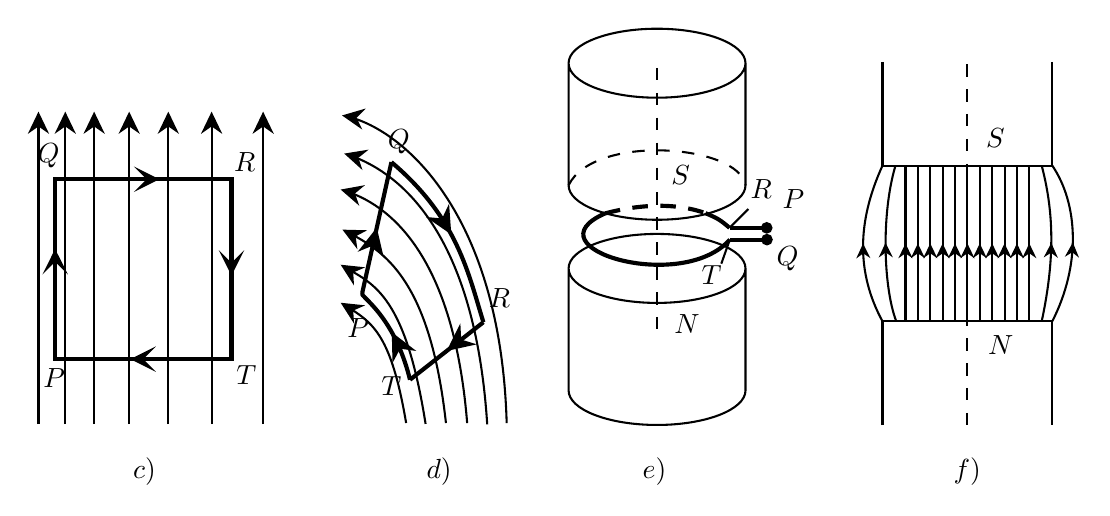
\begin{tikzpicture}[x=0.75pt,y=0.75pt,yscale=-1,xscale=1]
%uncomment if require: \path (0,508); %set diagram left start at 0, and has height of 508

%Curve Lines [id:da17704119093765347] 
\draw    (265.22,236.28) .. controls (262.37,135.31) and (215.55,95.15) .. (188.73,88.59) ;
\draw [shift={(185.9,88.01)}, rotate = 369.33000000000004] [fill={rgb, 255:red, 0; green, 0; blue, 0 }  ][line width=0.08]  [draw opacity=0] (10.72,-5.15) -- (0,0) -- (10.72,5.15) -- (7.12,0) -- cycle    ;
%Shape: Rectangle [id:dp2836649028479259] 
\draw  [line width=1.5]  (47.59,118.54) -- (132.66,118.54) -- (132.66,205.43) -- (47.59,205.43) -- cycle ;
\draw  [fill={rgb, 255:red, 0; green, 0; blue, 0 }  ,fill opacity=1 ] (88.13,114.41) -- (96.8,118.75) -- (88.13,123.08) -- (92.46,118.75) -- cycle ;
\draw  [fill={rgb, 255:red, 0; green, 0; blue, 0 }  ,fill opacity=1 ] (136.96,155.39) -- (132.63,164.06) -- (128.29,155.39) -- (132.63,159.73) -- cycle ;
\draw  [fill={rgb, 255:red, 0; green, 0; blue, 0 }  ,fill opacity=1 ] (93.71,209.74) -- (85.04,205.41) -- (93.71,201.07) -- (89.37,205.41) -- cycle ;
\draw  [fill={rgb, 255:red, 0; green, 0; blue, 0 }  ,fill opacity=1 ] (43.33,162.14) -- (47.66,153.47) -- (52,162.14) -- (47.66,157.81) -- cycle ;
%Straight Lines [id:da7848944881489814] 
\draw    (39.64,236.71) -- (39.64,89.18) ;
\draw [shift={(39.64,86.18)}, rotate = 450] [fill={rgb, 255:red, 0; green, 0; blue, 0 }  ][line width=0.08]  [draw opacity=0] (10.72,-5.15) -- (0,0) -- (10.72,5.15) -- (7.12,0) -- cycle    ;
%Straight Lines [id:da7900679033699884] 
\draw    (52.55,236.71) -- (52.55,89.18) ;
\draw [shift={(52.55,86.18)}, rotate = 450] [fill={rgb, 255:red, 0; green, 0; blue, 0 }  ][line width=0.08]  [draw opacity=0] (10.72,-5.15) -- (0,0) -- (10.72,5.15) -- (7.12,0) -- cycle    ;
%Straight Lines [id:da8748247138522687] 
\draw    (66.46,236.71) -- (66.46,89.18) ;
\draw [shift={(66.46,86.18)}, rotate = 450] [fill={rgb, 255:red, 0; green, 0; blue, 0 }  ][line width=0.08]  [draw opacity=0] (10.72,-5.15) -- (0,0) -- (10.72,5.15) -- (7.12,0) -- cycle    ;
%Straight Lines [id:da14628756799680054] 
\draw    (83.34,236.71) -- (83.34,89.18) ;
\draw [shift={(83.34,86.18)}, rotate = 450] [fill={rgb, 255:red, 0; green, 0; blue, 0 }  ][line width=0.08]  [draw opacity=0] (10.72,-5.15) -- (0,0) -- (10.72,5.15) -- (7.12,0) -- cycle    ;
%Straight Lines [id:da7920165637776044] 
\draw    (102.2,236.71) -- (102.2,89.18) ;
\draw [shift={(102.2,86.18)}, rotate = 450] [fill={rgb, 255:red, 0; green, 0; blue, 0 }  ][line width=0.08]  [draw opacity=0] (10.72,-5.15) -- (0,0) -- (10.72,5.15) -- (7.12,0) -- cycle    ;
%Straight Lines [id:da7403220227482121] 
\draw    (123.06,236.71) -- (123.06,89.18) ;
\draw [shift={(123.06,86.18)}, rotate = 450] [fill={rgb, 255:red, 0; green, 0; blue, 0 }  ][line width=0.08]  [draw opacity=0] (10.72,-5.15) -- (0,0) -- (10.72,5.15) -- (7.12,0) -- cycle    ;
%Straight Lines [id:da018032475368297662] 
\draw    (147.88,236.71) -- (147.88,89.18) ;
\draw [shift={(147.88,86.18)}, rotate = 450] [fill={rgb, 255:red, 0; green, 0; blue, 0 }  ][line width=0.08]  [draw opacity=0] (10.72,-5.15) -- (0,0) -- (10.72,5.15) -- (7.12,0) -- cycle    ;
%Curve Lines [id:da2082178622856372] 
\draw    (255.84,236.82) .. controls (249.84,143.51) and (213.08,115.42) .. (189.79,107.29) ;
\draw [shift={(186.95,106.38)}, rotate = 376.5] [fill={rgb, 255:red, 0; green, 0; blue, 0 }  ][line width=0.08]  [draw opacity=0] (10.72,-5.15) -- (0,0) -- (10.72,5.15) -- (7.12,0) -- cycle    ;
%Curve Lines [id:da017834833495530278] 
\draw    (246.18,236.21) .. controls (240.01,159.72) and (212.02,132.44) .. (187.86,124.5) ;
\draw [shift={(185.24,123.71)}, rotate = 375.41999999999996] [fill={rgb, 255:red, 0; green, 0; blue, 0 }  ][line width=0.08]  [draw opacity=0] (10.72,-5.15) -- (0,0) -- (10.72,5.15) -- (7.12,0) -- cycle    ;
%Curve Lines [id:da12164480539055833] 
\draw    (235.96,236.21) .. controls (228.26,166.71) and (205.96,153.24) .. (188.77,144.39) ;
\draw [shift={(186.1,143.03)}, rotate = 387.12] [fill={rgb, 255:red, 0; green, 0; blue, 0 }  ][line width=0.08]  [draw opacity=0] (10.72,-5.15) -- (0,0) -- (10.72,5.15) -- (7.12,0) -- cycle    ;
%Curve Lines [id:da6645218417107026] 
\draw    (226.15,236.64) .. controls (216.49,175.43) and (201.5,169.39) .. (187.65,161.36) ;
\draw [shift={(185.24,159.93)}, rotate = 391.7] [fill={rgb, 255:red, 0; green, 0; blue, 0 }  ][line width=0.08]  [draw opacity=0] (10.72,-5.15) -- (0,0) -- (10.72,5.15) -- (7.12,0) -- cycle    ;
%Curve Lines [id:da1770395852854001] 
\draw    (216.78,236.21) .. controls (209.57,193.75) and (200.85,187.81) .. (187.8,179.82) ;
\draw [shift={(185.24,178.25)}, rotate = 391.7] [fill={rgb, 255:red, 0; green, 0; blue, 0 }  ][line width=0.08]  [draw opacity=0] (10.72,-5.15) -- (0,0) -- (10.72,5.15) -- (7.12,0) -- cycle    ;
%Straight Lines [id:da7881452227089873] 
\draw [line width=1.5]    (195.61,173.57) -- (209.68,110.5) ;
\draw [shift={(202.64,142.03)}, rotate = 462.57] [fill={rgb, 255:red, 0; green, 0; blue, 0 }  ][line width=0.08]  [draw opacity=0] (13.4,-6.43) -- (0,0) -- (13.4,6.44) -- (8.9,0) -- cycle    ;
%Straight Lines [id:da8722762316049659] 
\draw [line width=1.5]    (254,187.63) -- (218.63,215.33) ;
\draw [shift={(236.31,201.48)}, rotate = 321.93] [fill={rgb, 255:red, 0; green, 0; blue, 0 }  ][line width=0.08]  [draw opacity=0] (13.4,-6.43) -- (0,0) -- (13.4,6.44) -- (8.9,0) -- cycle    ;
%Curve Lines [id:da3404753175974746] 
\draw [line width=1.5]    (209.68,110.5) .. controls (241.64,137.49) and (246.75,164.33) .. (254,187.63) ;
\draw [shift={(238.53,145.36)}, rotate = 240.23] [fill={rgb, 255:red, 0; green, 0; blue, 0 }  ][line width=0.08]  [draw opacity=0] (13.4,-6.43) -- (0,0) -- (13.4,6.44) -- (8.9,0) -- cycle    ;
%Curve Lines [id:da6848625095228247] 
\draw [line width=1.5]    (218.63,215.33) .. controls (210.81,183.37) and (193.77,174.85) .. (195.61,173.57) ;
\draw [shift={(209.86,192.46)}, rotate = 423] [fill={rgb, 255:red, 0; green, 0; blue, 0 }  ][line width=0.08]  [draw opacity=0] (13.4,-6.43) -- (0,0) -- (13.4,6.44) -- (8.9,0) -- cycle    ;
%Shape: Can [id:dp53613609777672] 
\draw   (380.28,161.71) -- (380.28,220.51) .. controls (380.28,229.69) and (361.2,237.13) .. (337.66,237.13) .. controls (314.13,237.13) and (295.05,229.69) .. (295.05,220.51) -- (295.05,161.71) .. controls (295.05,152.53) and (314.13,145.09) .. (337.66,145.09) .. controls (361.2,145.09) and (380.28,152.53) .. (380.28,161.71) .. controls (380.28,170.88) and (361.2,178.33) .. (337.66,178.33) .. controls (314.13,178.33) and (295.05,170.88) .. (295.05,161.71) ;
%Shape: Can [id:dp8542117011968777] 
\draw   (380.28,62.84) -- (380.28,121.65) .. controls (380.28,130.83) and (361.2,138.27) .. (337.66,138.27) .. controls (314.13,138.27) and (295.05,130.83) .. (295.05,121.65) -- (295.05,62.84) .. controls (295.05,53.66) and (314.13,46.22) .. (337.66,46.22) .. controls (361.2,46.22) and (380.28,53.66) .. (380.28,62.84) .. controls (380.28,72.02) and (361.2,79.46) .. (337.66,79.46) .. controls (314.13,79.46) and (295.05,72.02) .. (295.05,62.84) ;
%Curve Lines [id:da32502879442347266] 
\draw  [dash pattern={on 4.5pt off 4.5pt}]  (295.05,121.65) .. controls (307.12,96.72) and (377.01,101.83) .. (380.28,121.65) ;
%Curve Lines [id:da1758573324067343] 
\draw [line width=1.5]    (312.55,135.23) .. controls (274.88,151.93) and (349.54,174.09) .. (372.72,147.84) ;
%Curve Lines [id:da6169696982999335] 
\draw [line width=1.5]  [dash pattern={on 5.63pt off 4.5pt}]  (312.55,135.23) .. controls (333.4,129.66) and (349.77,131.02) .. (361.02,135.11) ;
%Curve Lines [id:da5111363917151119] 
\draw [line width=1.5]    (361.02,135.11) .. controls (366.47,137.39) and (367.83,138.07) .. (372.61,142.16) ;
%Straight Lines [id:da8337715960430991] 
\draw [line width=1.5]    (372.61,142.16) -- (390.51,142.16) ;
\draw [shift={(390.51,142.16)}, rotate = 0] [color={rgb, 255:red, 0; green, 0; blue, 0 }  ][fill={rgb, 255:red, 0; green, 0; blue, 0 }  ][line width=1.5]      (0, 0) circle [x radius= 1.74, y radius= 1.74]   ;
%Straight Lines [id:da9610326272369787] 
\draw [line width=1.5]    (372.72,147.84) -- (390.62,147.84) ;
\draw [shift={(390.62,147.84)}, rotate = 0] [color={rgb, 255:red, 0; green, 0; blue, 0 }  ][fill={rgb, 255:red, 0; green, 0; blue, 0 }  ][line width=1.5]      (0, 0) circle [x radius= 1.74, y radius= 1.74]   ;
%Straight Lines [id:da11384148043546372] 
\draw    (372.61,142.16) -- (381.66,133.11) ;
%Straight Lines [id:da20341759509474677] 
\draw    (372.72,147.84) -- (368.63,159.43) ;
%Straight Lines [id:da6004574358455221] 
\draw  [dash pattern={on 4.5pt off 4.5pt}]  (337.66,65.11) -- (337.66,196.08) ;
%Shape: Right Angle [id:dp21523229649023556] 
\draw   (528.1,62.18) -- (528.1,112.18) -- (446.28,112.18) ;
%Shape: Right Angle [id:dp06070969519937974] 
\draw   (446.28,237.18) -- (446.28,187.18) -- (528.1,187.18) ;
%Straight Lines [id:da46072993739083357] 
\draw    (528.1,187.18) -- (528.1,237.18) ;
%Straight Lines [id:da7394340970219537] 
\draw    (446.28,62.18) -- (446.28,112.18) ;
%Straight Lines [id:da11637676650266049] 
\draw  [dash pattern={on 4.5pt off 4.5pt}]  (487.19,63.31) -- (487.19,241.35) ;
%Straight Lines [id:da8977810319571025] 
\draw    (517.02,187.18) -- (517.02,112.18) ;
\draw [shift={(517.02,149.68)}, rotate = 450] [fill={rgb, 255:red, 0; green, 0; blue, 0 }  ][line width=0.08]  [draw opacity=0] (7.14,-3.43) -- (0,0) -- (7.14,3.43) -- (4.74,0) -- cycle    ;
%Straight Lines [id:da3058576723356914] 
\draw    (511.06,187.18) -- (511.06,112.18) ;
\draw [shift={(511.06,149.68)}, rotate = 450] [fill={rgb, 255:red, 0; green, 0; blue, 0 }  ][line width=0.08]  [draw opacity=0] (7.14,-3.43) -- (0,0) -- (7.14,3.43) -- (4.74,0) -- cycle    ;
%Straight Lines [id:da4173412375926153] 
\draw    (505.09,187.18) -- (505.09,112.18) ;
\draw [shift={(505.09,149.68)}, rotate = 450] [fill={rgb, 255:red, 0; green, 0; blue, 0 }  ][line width=0.08]  [draw opacity=0] (7.14,-3.43) -- (0,0) -- (7.14,3.43) -- (4.74,0) -- cycle    ;
%Straight Lines [id:da9461491818536378] 
\draw    (499.13,187.18) -- (499.13,112.18) ;
\draw [shift={(499.13,149.68)}, rotate = 450] [fill={rgb, 255:red, 0; green, 0; blue, 0 }  ][line width=0.08]  [draw opacity=0] (7.14,-3.43) -- (0,0) -- (7.14,3.43) -- (4.74,0) -- cycle    ;
%Straight Lines [id:da1656452678084357] 
\draw    (493.16,187.18) -- (493.16,112.18) ;
\draw [shift={(493.16,149.68)}, rotate = 450] [fill={rgb, 255:red, 0; green, 0; blue, 0 }  ][line width=0.08]  [draw opacity=0] (7.14,-3.43) -- (0,0) -- (7.14,3.43) -- (4.74,0) -- cycle    ;
%Straight Lines [id:da9719949783410846] 
\draw    (487.19,187.18) -- (487.19,112.18) ;
\draw [shift={(487.19,149.68)}, rotate = 450] [fill={rgb, 255:red, 0; green, 0; blue, 0 }  ][line width=0.08]  [draw opacity=0] (7.14,-3.43) -- (0,0) -- (7.14,3.43) -- (4.74,0) -- cycle    ;
%Straight Lines [id:da45818028238885855] 
\draw    (481.23,187.18) -- (481.23,112.18) ;
\draw [shift={(481.23,149.68)}, rotate = 450] [fill={rgb, 255:red, 0; green, 0; blue, 0 }  ][line width=0.08]  [draw opacity=0] (7.14,-3.43) -- (0,0) -- (7.14,3.43) -- (4.74,0) -- cycle    ;
%Straight Lines [id:da8303819650972852] 
\draw    (475.26,187.18) -- (475.26,112.18) ;
\draw [shift={(475.26,149.68)}, rotate = 450] [fill={rgb, 255:red, 0; green, 0; blue, 0 }  ][line width=0.08]  [draw opacity=0] (7.14,-3.43) -- (0,0) -- (7.14,3.43) -- (4.74,0) -- cycle    ;
%Straight Lines [id:da4551447016455965] 
\draw    (469.3,187.18) -- (469.3,112.18) ;
\draw [shift={(469.3,149.68)}, rotate = 450] [fill={rgb, 255:red, 0; green, 0; blue, 0 }  ][line width=0.08]  [draw opacity=0] (7.14,-3.43) -- (0,0) -- (7.14,3.43) -- (4.74,0) -- cycle    ;
%Straight Lines [id:da594753385683483] 
\draw    (463.33,187.18) -- (463.33,112.18) ;
\draw [shift={(463.33,149.68)}, rotate = 450] [fill={rgb, 255:red, 0; green, 0; blue, 0 }  ][line width=0.08]  [draw opacity=0] (7.14,-3.43) -- (0,0) -- (7.14,3.43) -- (4.74,0) -- cycle    ;
%Straight Lines [id:da7016635346218927] 
\draw    (457.36,187.18) -- (457.36,112.18) ;
\draw [shift={(457.36,149.68)}, rotate = 450] [fill={rgb, 255:red, 0; green, 0; blue, 0 }  ][line width=0.08]  [draw opacity=0] (7.14,-3.43) -- (0,0) -- (7.14,3.43) -- (4.74,0) -- cycle    ;
%Curve Lines [id:da06981159388742642] 
\draw    (452.84,186.99) .. controls (446.69,170.62) and (445.62,135.46) .. (452.5,112.33) ;
\draw [shift={(447.77,149.3)}, rotate = 449.2] [fill={rgb, 255:red, 0; green, 0; blue, 0 }  ][line width=0.08]  [draw opacity=0] (7.14,-3.43) -- (0,0) -- (7.14,3.43) -- (4.74,0) -- cycle    ;
%Curve Lines [id:da16396718213086392] 
\draw    (446.28,187.18) .. controls (433.48,163.59) and (434.11,138.87) .. (446.28,112.18) ;
\draw [shift={(436.93,149.72)}, rotate = 448.92] [fill={rgb, 255:red, 0; green, 0; blue, 0 }  ][line width=0.08]  [draw opacity=0] (7.14,-3.43) -- (0,0) -- (7.14,3.43) -- (4.74,0) -- cycle    ;
%Curve Lines [id:da36261811968074475] 
\draw    (528.1,187.18) .. controls (541.93,159.97) and (540.65,130.77) .. (528.1,112.18) ;
\draw [shift={(537.98,149.2)}, rotate = 453.47] [fill={rgb, 255:red, 0; green, 0; blue, 0 }  ][line width=0.08]  [draw opacity=0] (7.14,-3.43) -- (0,0) -- (7.14,3.43) -- (4.74,0) -- cycle    ;
%Curve Lines [id:da2084422404430566] 
\draw    (522.99,187.18) .. controls (529.78,155.49) and (528.51,133.33) .. (522.99,112.18) ;
\draw [shift={(527.61,149.41)}, rotate = 451.86] [fill={rgb, 255:red, 0; green, 0; blue, 0 }  ][line width=0.08]  [draw opacity=0] (7.14,-3.43) -- (0,0) -- (7.14,3.43) -- (4.74,0) -- cycle    ;

% Text Node
\draw (37.68,100.13) node [anchor=north west][inner sep=0.75pt]    {$Q$};
% Text Node
\draw (132.44,104.39) node [anchor=north west][inner sep=0.75pt]    {$R$};
% Text Node
\draw (40.46,208.37) node [anchor=north west][inner sep=0.75pt]    {$P$};
% Text Node
\draw (133.48,207.2) node [anchor=north west][inner sep=0.75pt]    {$T$};
% Text Node
\draw (186.91,184.29) node [anchor=north west][inner sep=0.75pt]    {$P$};
% Text Node
\draw (206.44,93.31) node [anchor=north west][inner sep=0.75pt]    {$Q$};
% Text Node
\draw (255.17,170.02) node [anchor=north west][inner sep=0.75pt]    {$R$};
% Text Node
\draw (203.36,212.32) node [anchor=north west][inner sep=0.75pt]    {$T$};
% Text Node
\draw (343.03,110.64) node [anchor=north west][inner sep=0.75pt]    {$S$};
% Text Node
\draw (344.51,182.23) node [anchor=north west][inner sep=0.75pt]    {$N$};
% Text Node
\draw (396.72,122.29) node [anchor=north west][inner sep=0.75pt]    {$P$};
% Text Node
\draw (393.77,149.62) node [anchor=north west][inner sep=0.75pt]    {$Q$};
% Text Node
\draw (357.63,158.62) node [anchor=north west][inner sep=0.75pt]    {$T$};
% Text Node
\draw (381.31,117.46) node [anchor=north west][inner sep=0.75pt]    {$R$};
% Text Node
\draw (495.65,192.74) node [anchor=north west][inner sep=0.75pt]    {$N$};
% Text Node
\draw (494.74,92.74) node [anchor=north west][inner sep=0.75pt]    {$S$};
% Text Node
\draw (83.78,251.55) node [anchor=north west][inner sep=0.75pt]    {$c)$};
% Text Node
\draw (225.11,251.55) node [anchor=north west][inner sep=0.75pt]    {$d)$};
% Text Node
\draw (329.24,251.55) node [anchor=north west][inner sep=0.75pt]    {$e)$};
% Text Node
\draw (479.03,251.55) node [anchor=north west][inner sep=0.75pt]    {$f)$};
\end{tikzpicture}
    \end{center}
\begin{enumerate}[1)]
    \item 
    Hình $c)$ biểu diễn các đường sức của một điện trường hướng từ dưới lên: dọc theo một đường sức thì điện trường có độ lớn không đổi, còn từ trái sang thì điện trường yếu dần, các đường sức là những đường thẳng song song nhưng từ trái sang thì chúng thưa dần. Hãy áp dụng (\ref{q.d.1}) với một hình chữ nhật $PQRT$ có cạnh $PQ$ song song với các đường sức để chứng minh rằng một điện trường như mô tả không thể tồn tại nếu tại đó không có từ trường biến thiên theo thời gian. Như vậy, nếu các đường sức là các đường thẳng thì chúng phải nằm cách đều nhau. Kết quả này có thể giải thích như là các đường sức dường như đẩy nhau và các đường sức song song phải sắp xếp sao cho chúng cách đều nhau.
    \item Trên hình $d)$, các đường sức là những cung tròn đồng tâm cách đều nhau. Dọc theo một đường sức điện trường đổi hướng nhưng có độ lớn không đổi. Áp dụng (\ref{q.d.1}) với đường cong kín $PQRT$ có cạnh $\overrightarrow{PQ}$ và $\overrightarrow{RT}$ vuông góc với các đường sức từ và ${PT},{RQ}$ là các cung tròn đồng tâm với các đường sức. Chứng minh rằng độ lớn của điện trường tại một điểm tỷ lệ nghịch với khoảng cách tới tâm nếu trong vùng đang xét không có từ trường biến thiên.\\
    Trên hình $e)$, hai cực Bắc $(N)$ và Nam $(S)$ của một nam châm điện có dạng hình trụ và làm từ vật liệu đồng nhất được đặt cách nhau tạo thành một khe hẹp. Từ trường giữa hai cực nam châm ở vùng gần tâm là đều và các đường sức từ vuông góc với các cực như hình $f)$. Bằng cách thay đổi cường độ các dòng điện tròn bao quanh các cực nam châm và người ta có thể tạo ra các từ trường biến thiên. Các đường sức điện cảm ứng có dạng các đường tròn có tâm nằm trên trục nam châm. Áp dụng (\ref{q.d.1}) với đường cong kín ${C}$ là một đường tròn nằm trong mặt phẳng vuông góc với các đường sức và có tâm nằm trên trục nam châm, mặt ${S}$ là mặt phẳng giới hạn bởi đường cong ${C}$ này.
    \item Chọn chiều dương của từ trường ${B}({t})$ từ cực Bắc về Nam, khi đó điện trường tại một điểm cách tâm một khoảng ${r}$ sẽ là:
\[E({t})=-\dfrac{r}{2} \dfrac{\Delta B({t})}{\Delta t}.\tag{2}\label{q.d.2}\]
Trong đó: ${E}({t})$ mang dấu dương nếu nó chạy ngược chiều kim đồng hồ khi nhìn từ cực ${S}$. Tiếp theo, khi một khung dây được đưa vào khe và nối ra ngoài qua hai cực ${P}, {Q}$. Hãy tìm hiệu điện thế giữa hai điểm $Q$ và $P$, biết rằng bán kính của khung dây tròn là $r$ và coi rằng khe $RT$ có kích thước nhỏ hơn rất nhiều chu vi của vòng.
\item Bây giờ người ta bỏ khung dây đi và tại một điểm cách trục nam châm một khoảng $R$, người ta đặt vào một điện tích $q$. Khi từ trường trong khe biến thiên, điện tích chuyển động dưới tác dụng của lực điện trường cảm ứng gây ra bởi từ trường. Xét trường hợp điện tích chuyển động trên một đường tròn cố định.\\
Kí hiệu ${E}({t})$ là điện trường của đường sức điện hình tròn bán kính ${R}$ và có tâm nằm trên trục nam châm. Ngoài ra ${B}({t})$ là cảm ứng từ. Đầu tiên hãy coi hai đại lượng này là độc lập, hãy thiết lập mối quan hệ giữa ${E}({t})$ và ${B}({t})$ để điện tích $q$ chuyển động trên đường tròn bán kính $R$. Quy ước chiều dương hướng từ tâm vòng tròn ra phía ngoài và chiều dương của khung tròn là ngược chiều kim đồng hồ khi nhìn từ cực ${S}$.\\
Gợi ý: Khi hạt có vận tốc tức thời $v$, hãy viết phương trình chuyển động của hạt thông qua $\dfrac{\Delta v}{\Delta t}$.
\item Quan hệ giữa điện trường và từ trường vừa nhận được khác với kết quả của câu $3)$, khi mà từ trường giữa hai cực nam châm là đều. Như vậy, ta cần một từ trường và điện trường phụ có giá trị phụ thuộc cả vào khoảng cách tới tâm và thời gian là ${{E}(r}, {t})$ và ${B}({r}, {t})$. Ngoài ra, giả sử rằng cảm ứng từ có thể biểu diễn dưới dạng ${B}({r}, {t}) = {F}_{{B}}({r}) {G}({t})$. Tương tự từ thông gửi qua một mặt tròn bán kính ${r}$ sẽ là $\Phi({r}, {t}) = {F}_{\Phi}({r}) {G}({t})$. Hãy xét đường tròn bán kính ${r}={R}$ và chứng minh:
\[F_{\Phi}(R) = 2 \pi R^{2} F_{B}({R})\tag{3}\label{q.d.3} \]
\item Để tạo ra từ trường thỏa mãn điều kiện ở câu trên, người ta dùng hai cuộn dây solenoid đặt đồng trục thay vì nam châm điện. Gọi $a$ và $b$ lần lượt là bán kính của các cuộn dây đặt ngoài và trong. Mật độ vòng dây trên hai cuộn là như nhau. Dòng điện chạy qua các cuộn dây có cùng chiều nhưng cường độ dòng chạy ở cuộn trong lớn gấp đôi cường độ dòng chạy ở cuộn ngoài. Hãy tìm bán kính các cuộn dây theo ${R}$ để các điều kiện (\ref{q.d.3}) ở trên thỏa mãn.\\

\item Giữa điện trường và từ trường biến thiên, ngoài điều kiện (\ref{q.d.1}) ở trên, quan hệ sau được thỏa mãn:
\[V_{m}(C)=\frac{\Delta \Phi(S)}{\Delta t}. \tag{4}\label{q.d.4}\]
Phương trình (\ref{q.d.4}) này có dạng giống phương trình (\ref{q.d.1}), ngoại trừ việc thiếu dấu trừ ở vế phải.\\
Để hiểu rõ hơn về phương trình (\ref{q.d.4}), hãy xét một mặt $S$ được giới hạn bởi đường cong kín $C$. Tuy nhiên, khác với hình ${a})$, qua mặt ${S}$ của đường cong kín ${C}$ bây giờ sẽ là điện thông $\Phi_{e}$ thay vì từ thông. Mọi tính toán hoàn toàn tương tự như của trường hợp từ trường, ngoại trừ vector cảm ứng từ $\ot{B}$ bây giờ sẽ được thay thế bởi vector cảm ứng điện $\ot{D} = \varepsilon_{0} \ot{E}$. Ngoài ra, để tính sức từ động cảm ứng $V_{m}(C)$ theo đường cong kín ${C}$ bây giờ ta phải thay cường độ điện trường $\ot{E}$ bằng cường độ từ trường, được định nghĩa: $\ot{H} = \dfrac{\ot{B}}{\mu_{0}}$.\\
Ở đây, $\varepsilon_{0}$ và $\mu_{0}$ lần lượt là hằng số điện và độ điện cảm chân không (hằng số từ). Ngoài ra, dấu của điện thông qua đường cong kín ${C}$ được xác định như trong trường hợp từ thông.\\
Xét một tụ điện phẳng mà hai bản tụ có dạng đĩa tròn, bán kính ${a}$, đặt song song đồng trục. Điện tích trên các bản tụ có thể thay đổi theo thời gian $\pm {Q}({t}),\tron{{Q}({t})>0}$. Khi điện tích thay đổi, các đường sức từ cảm ứng là các đường tròn có tâm nằm trên trục của tụ điện. Hãy tìm cảm ứng từ tại một điểm cách tâm một khoảng ${r} < {a}$. Khi điện tích ${Q}({t})$ tăng thì các đường sức từ quay theo chiều kim đồng hồ hay ngược chiều kim đồng hồ, nếu nhìn từ bản cực âm của tụ điện? Giả sử khoảng cách giữa hai bản tụ nhỏ hơn rất nhiều bán kính của chúng và bỏ qua mọi hiệu ứng rìa.
\end{enumerate}
\end{vd}
\begin{loigiai}
\begin{enumerate}[1)]
    \item Góc giữa phương của đường sức điện với các đoạn $\overline{QR}, \overline{TP}$  bằng ${{90}^{\circ}}$ nên suất điện động trên hai đoạn này đều bằng không. Trong khi đó, góc giữa đường sức với đoạn $\overline{PQ}$ bằng $0^\circ$ và với $\overline{RT}$ bằng $180^\circ$. Do đó, khi  $\overline{PQ}=\overline{RT}=l$, suất điện động trong khung dây ở hình $c)$ là
    \[{{V}_{PQRT}} = l\left( {{E}_{PQ}}-{{E}_{RT}} \right).\]
    Trong đó ${{E}_{PQ}}$ và ${{E}_{RT}}$ là độ lớn điện trường trên các đoạn $\overline{PQ}$ và $\overline{RT}$ tương ứng.\\ Nhưng vì suất điện động trên đường kín phải bằng không nên ${{E}_{PQ}} = {{E}_{RT}}$. Như vậy tại mọi điểm trong điện trường có đường sức song song thì cường độ điện trường có độ lớn như nhau.
    \item Trên các đoạn $\overline{PQ}$ và $\overline{RT}$ suất điện động bằng không. Độ dài cung $QR$ chắn đường tròn bán kính ${{r}_{1}}$ là ${{l}_{QR}}$. Độ dài cung $TP$ chắn đường tròn bán kính ${{r}_{2}}$ là ${{l}_{TR}}$ . Điện trường $\ot{E}$ tạo với $\overline{QR}$ góc $180^\circ$, và tạo với $\overline{TP}$ một góc $0^\circ$ nên suất điện động trên khung $PQRT$ là:
    \[{{V}_{PQRT}} = E({{r}_{2}}){{l}_{TP}} - E({{r}_{1}}){{l}_{QR}}.\]
    Không có từ trường biến thiên nên, từ phương trình (\ref{q.d.1}), suất điện động bằng không, suy ra \[\dfrac{E({{r}_{1}})}{E({{r}_{2}})}=\dfrac{{{l}_{TP}}}{{{l}_{QR}}} =\dfrac{{{r}_{2}}}{{{r}_{1}}},\] 
    tức là cường độ điện trường tỷ lệ nghịch với khoảng cách tới tâm.
    \item Áp dụng (\ref{q.d.1}) cho đường cong kín $C$ bán kính $r$. Diện tích chắn bởi đường tròn $\pi {{r}^{2}}$, từ thông gửi qua nó là $\Phi (t) = \pi {{r}^{2}}B(t)$. Như vậy vế phải của (\ref{q.d.1}) viết lại là 
    \[-\dfrac{\Delta \phi }{\Delta t}=-\pi {{r}^{2}}\dfrac{\Delta B(t)}{\Delta t}.\]
    Chu vi của đường sức điện trường tròn là $2\pi r$ vì điện trường tại mỗi điểm trên đường tròn đều tiếp tuyến với  đường tròn. Vế trái của (\ref{q.d.1}) là 
    \[V(C)=2\pi rE(t).\]
    Do đó, từ (\ref{q.d.1}) ta có:
    \[E(t) = -\dfrac{r}{2}\dfrac{\Delta B(t)}{\Delta t} < 0.\]  
    Khi khung dây nối với mạch ngoài, điện tích sẽ chạy từ $P$ rồi về $Q$ do đó cực $Q$ là âm, cực $P$ là dương.
    \[{{V}_{QP}} = -2\pi rE(t) = \pi {{r}^{2}}\dfrac{\Delta B(t)}{\Delta t}.\]
    \item  Gọi vận tốc của chất điểm là $v$, phương trình chuyển động trên chu vi đường tròn là 
    \[m\dfrac{\Delta v}{\Delta t} = qE(t).\tag{5}\label{q.d.5}\] 
    Điều kiện cân bằng lực ly tâm và lực lorentz:
    \[m\dfrac{{{v}^{2}}}{R}=-qvB(t)\tag{6}\label{q.d.6}.\]
    Giải hệ (\ref{q.d.5}) và (\ref{q.d.6}) ta được: \[E(t)=-R\dfrac{\Delta B(t)}{\Delta t}. \tag{7}\label{q.d.7}\]
    \item Trong biểu thức (\ref{q.d.1}) thay $r = R$ và phương trình trong đề bài, ta được: 
    \[2\pi R E(R,t) = -{{F}_{\Phi }}(R) \dfrac{\Delta G(t)}{\Delta t}. \tag{8}\label{q.d.8}\]
    Phương trình (\ref{q.d.7}) giờ trở thành
    \[E(R,t) = -R\dfrac{\Delta B(R,t)}{\Delta t} = -R{{F}_{B}}(R)\dfrac{\Delta G(t)}{\Delta t}. \tag{9}\label{q.d.9}\]
    Từ hai phương trình cuối (\ref{q.d.8}) và (\ref{q.d.9}), loại trừ $E(R,t)$ ta sẽ được biểu thức cần chứng minh.
   \[F_{\Phi}(R) = 2 \pi R^{2} F_{B}({R}).\]
   \item Gọi $n$ là mật độ vòng dây ở cuộn solenoid ngoài, và cường độ dòng điện chạy trong nó là $I(t)$. Để nằm trong từ trường thì quỹ đạo tròn phải đặt vào vị trí $R<a$. Vì từ trường bên trong vùng của quỹ đạo $R$ không là hằng số nên cần phải đặt $R>b$. Mặt khác, theo điều kiện bài toán, trong vùng $a>r>b$, ta có: \[B(r,t)={{\mu }_{0}}nI(t),\] trong vùng $r<b$, ta có \[B(r,t)=3{{\mu }_{0}}nI(t).\] Như vậy $F_B(R) = \dfrac{{{\mu }_{0}}nI(t)}{G(t)}$.\\  
    Từ thông qua tiết diện tròn bán kính $R, b<R<a$ là
    \[\Phi(R,t) = \pi ({{R}^{2}}-{{b}^{2}}){{\mu }_{0}}nI(t)+3{{\mu }_{0}}\pi{{b}^{2}}nI(t) = \dfrac{R_\Phi(R)}{G(t)}.\] 
    Từ hai phương trình trên và từ (\ref{q.d.3}), sau khi thế vào và biến đổi, ta được
    \[\pi {{R}^{2}}{{\mu }_{0}}nI(t) =  2\pi {{b}^{2}}{{\mu }_{0}}nI(t) \rt b = \dfrac{R}{\sqrt{2}}.\]
    \item Trong biểu thức (\ref{q.d.2}) của câu hỏi $3)$ ta thay $E\to H; B\to D$  và bỏ dấu trừ ở vế phải
    \[H(t)=\dfrac{r}{2}\dfrac{\Delta D(t)}{\Delta t}.\] 
    Vì $\heva{H(t) &= \dfrac{B(t)}{{{\mu }_{0}}} \\ D(t) &= {{\varepsilon }_{0}} E(t) = \dfrac{Q(t)}{\pi {{a}^{2}}} }$  nên:
    \[B(t)={{\mu }_{0}}\frac{r}{2\pi {{a}^{2}}}\dfrac{\Delta Q(t)}{\Delta t}\]  
    Vế phải phương trình này không chứa dấu trừ giống như trong biểu thức của điện trường cảm ứng ở câu hỏi $3)$, khi các cực $N$ và $S$ được thay bởi các điện cực dương và âm tương ứng, do đó nếu quan sát từ cực âm sẽ thấy đường sức ngược chiều kim đồng hồ.
\end{enumerate}
\end{loigiai}
